\chapter{Pandas}

\section{Introduction to pandas}
Pandas is an external library built on top of NumPy, designed for data analysis and manipulation. It is conventionally imported as \texttt{import pandas as pd}. 
pandas provides two primary data structures:

\begin{itemize}
    \item \textbf{Series:} A 1-dimensional column.
    \item \textbf{DataFrame:} A 2-dimensional table.
\end{itemize}
It replaces verbose plain Python loops and dictionaries with concise operations where row and column labels travel securely with the data.

\section{Series}

\subsection{Creation and Attributes}
A Series is a one-dimensional sequence of homogeneous elements. Unlike standard NumPy arrays, each element is associated with an explicit label within an \textbf{index} (which can be integers, strings, or dates).

\begin{figure}[h]
    \centering
    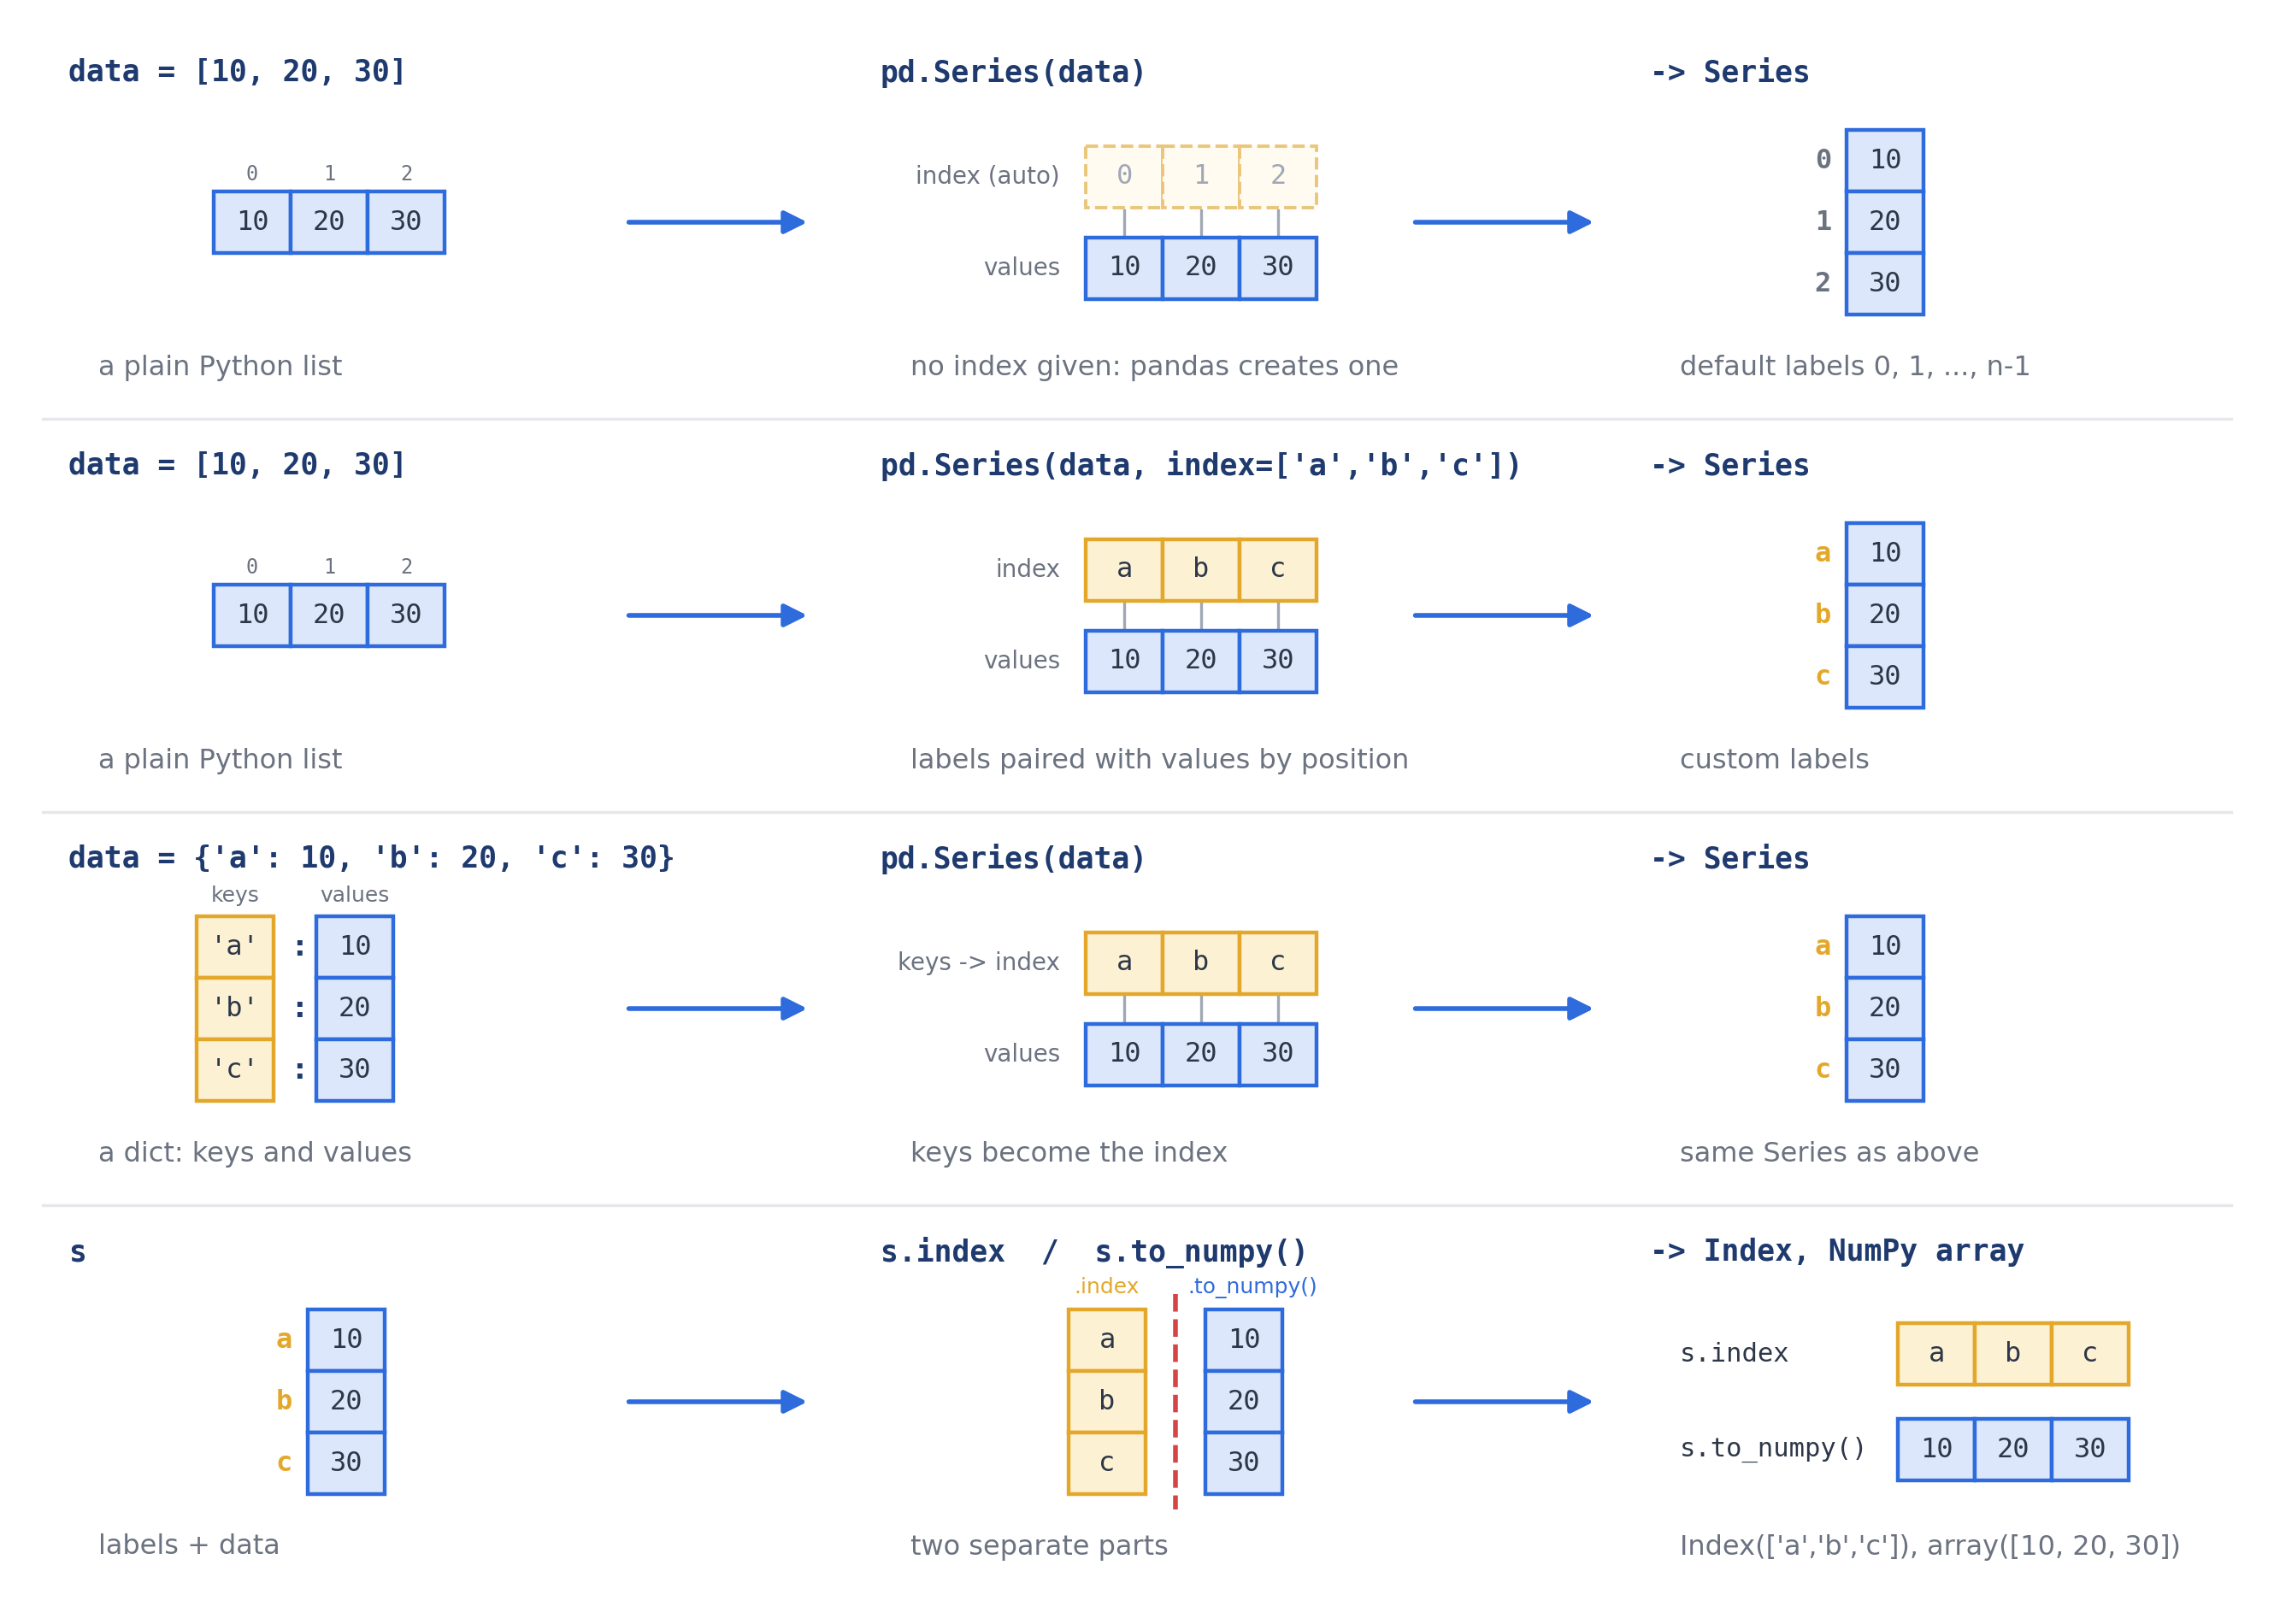
\includegraphics[width=1\textwidth]{contents/images/pandas/sub_series_creation.png}
    \caption{Creating a Series: from a list with the default index $0, \dots, n-1$, from a list with a custom \texttt{index}, and from a dictionary whose keys become the index. The attributes \texttt{.index} and \texttt{.to\_numpy()} return the labels and the data separately.}
\end{figure}

\begin{itemize}
    \item You can create a Series from a list (with or without specifying the \texttt{index} explicitly) or from a dictionary, where the keys automatically become the index.
    \item A Series acts as a NumPy array with labels: you can access the labels via the \texttt{.index} attribute and the raw array via the \texttt{.values} attribute.
\end{itemize}

\lstinputlisting[caption={Creating a Series and accessing its core attributes.}]{contents/listings/pandas/series_creation.py}

\subsection{Accessing Elements: \texttt{loc} vs \texttt{iloc}}
Because an integer can represent both a position and a label, pandas uses two distinct accessors to avoid ambiguity:
\begin{itemize}
    \item \texttt{.loc[label]}: Selects by \textbf{label} (the explicit name in the index). When slicing (\texttt{s.loc['a':'c']}), the stop element is \textbf{included}.
    \item \texttt{.iloc[position]}: Selects by \textbf{position} (0, 1, 2, ..., like standard Python lists). When slicing (\texttt{s.iloc[1:3]}), the stop element is \textbf{excluded}.
\end{itemize}

\begin{figure}[h]
    \centering
    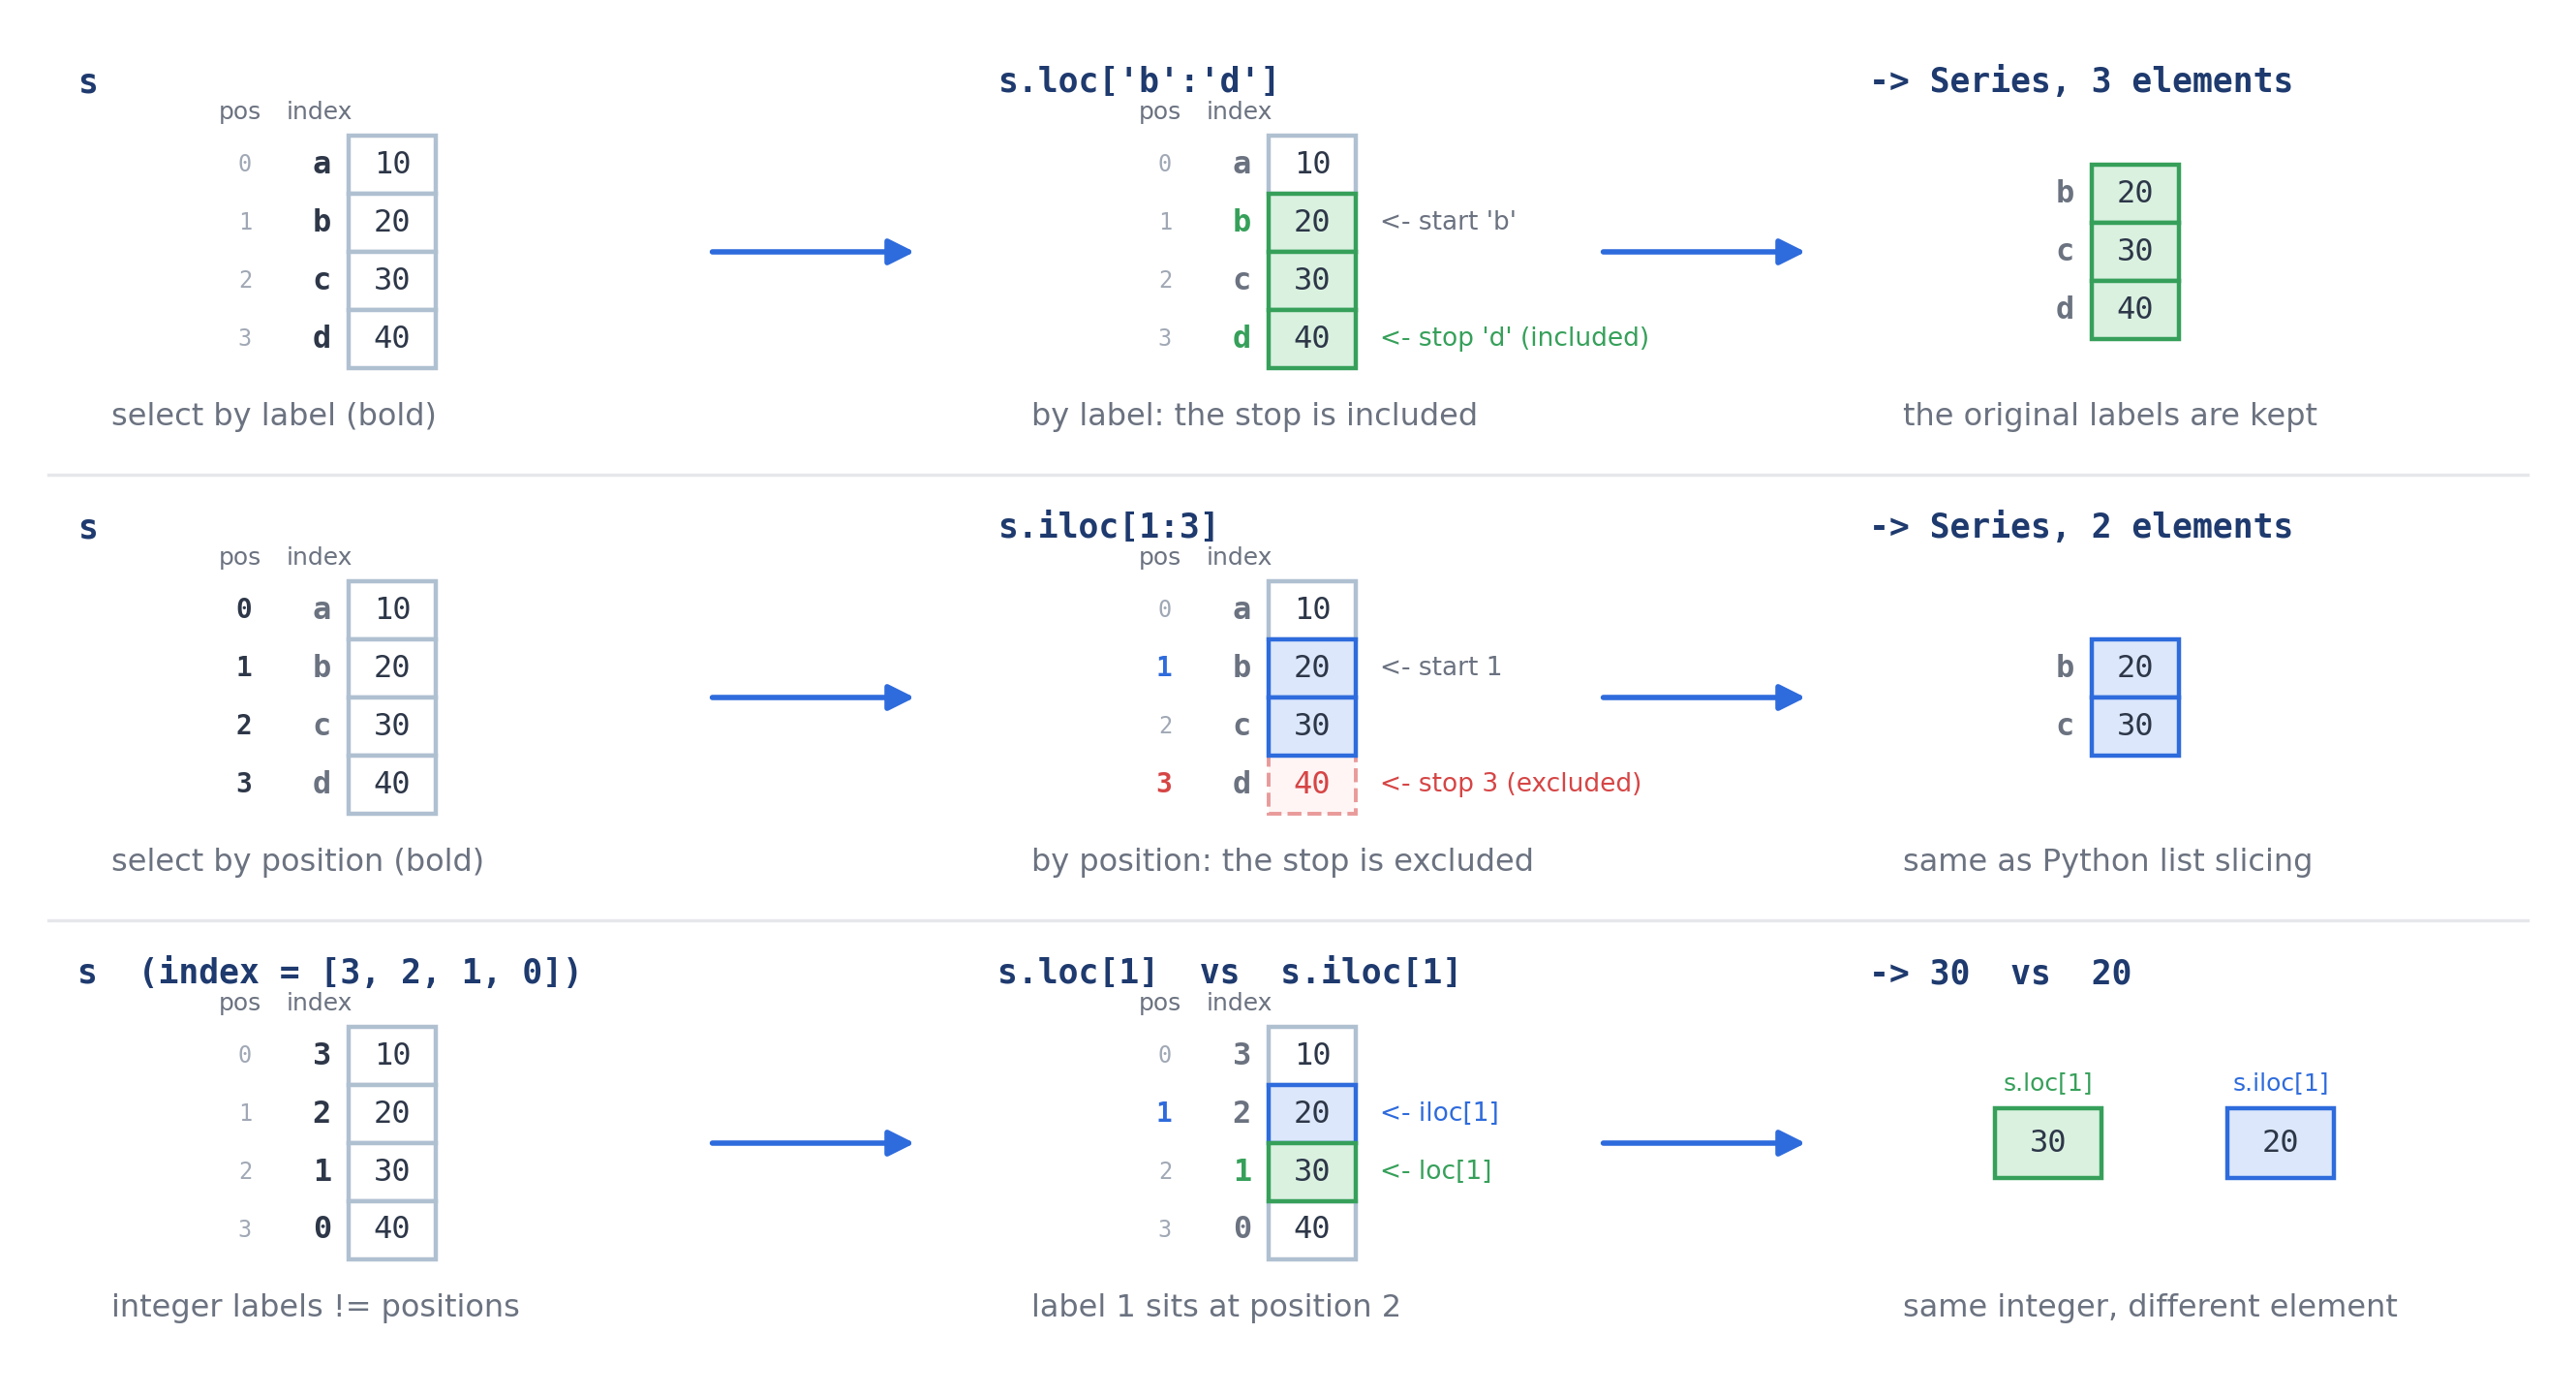
\includegraphics[width=1\textwidth]{contents/images/pandas/sub_loc_iloc.png}
    \caption{\texttt{loc} selects by label and includes the stop of a slice; \texttt{iloc} selects by position and excludes it. With integer labels, \texttt{s.loc[1]} and \texttt{s.iloc[1]} can return different elements.}
\end{figure}

\lstinputlisting[caption={Accessing Series elements using loc and iloc.}]{contents/listings/pandas/series_access.py}

\subsection{Masking and Fancy Indexing}

\begin{itemize}
    \item \textbf{Masking:} Applying a comparison to a Series creates a boolean mask. Because the mask is a Series itself containing labels, it must be used with \texttt{.loc}.
        \begin{figure}[h]
            \centering
            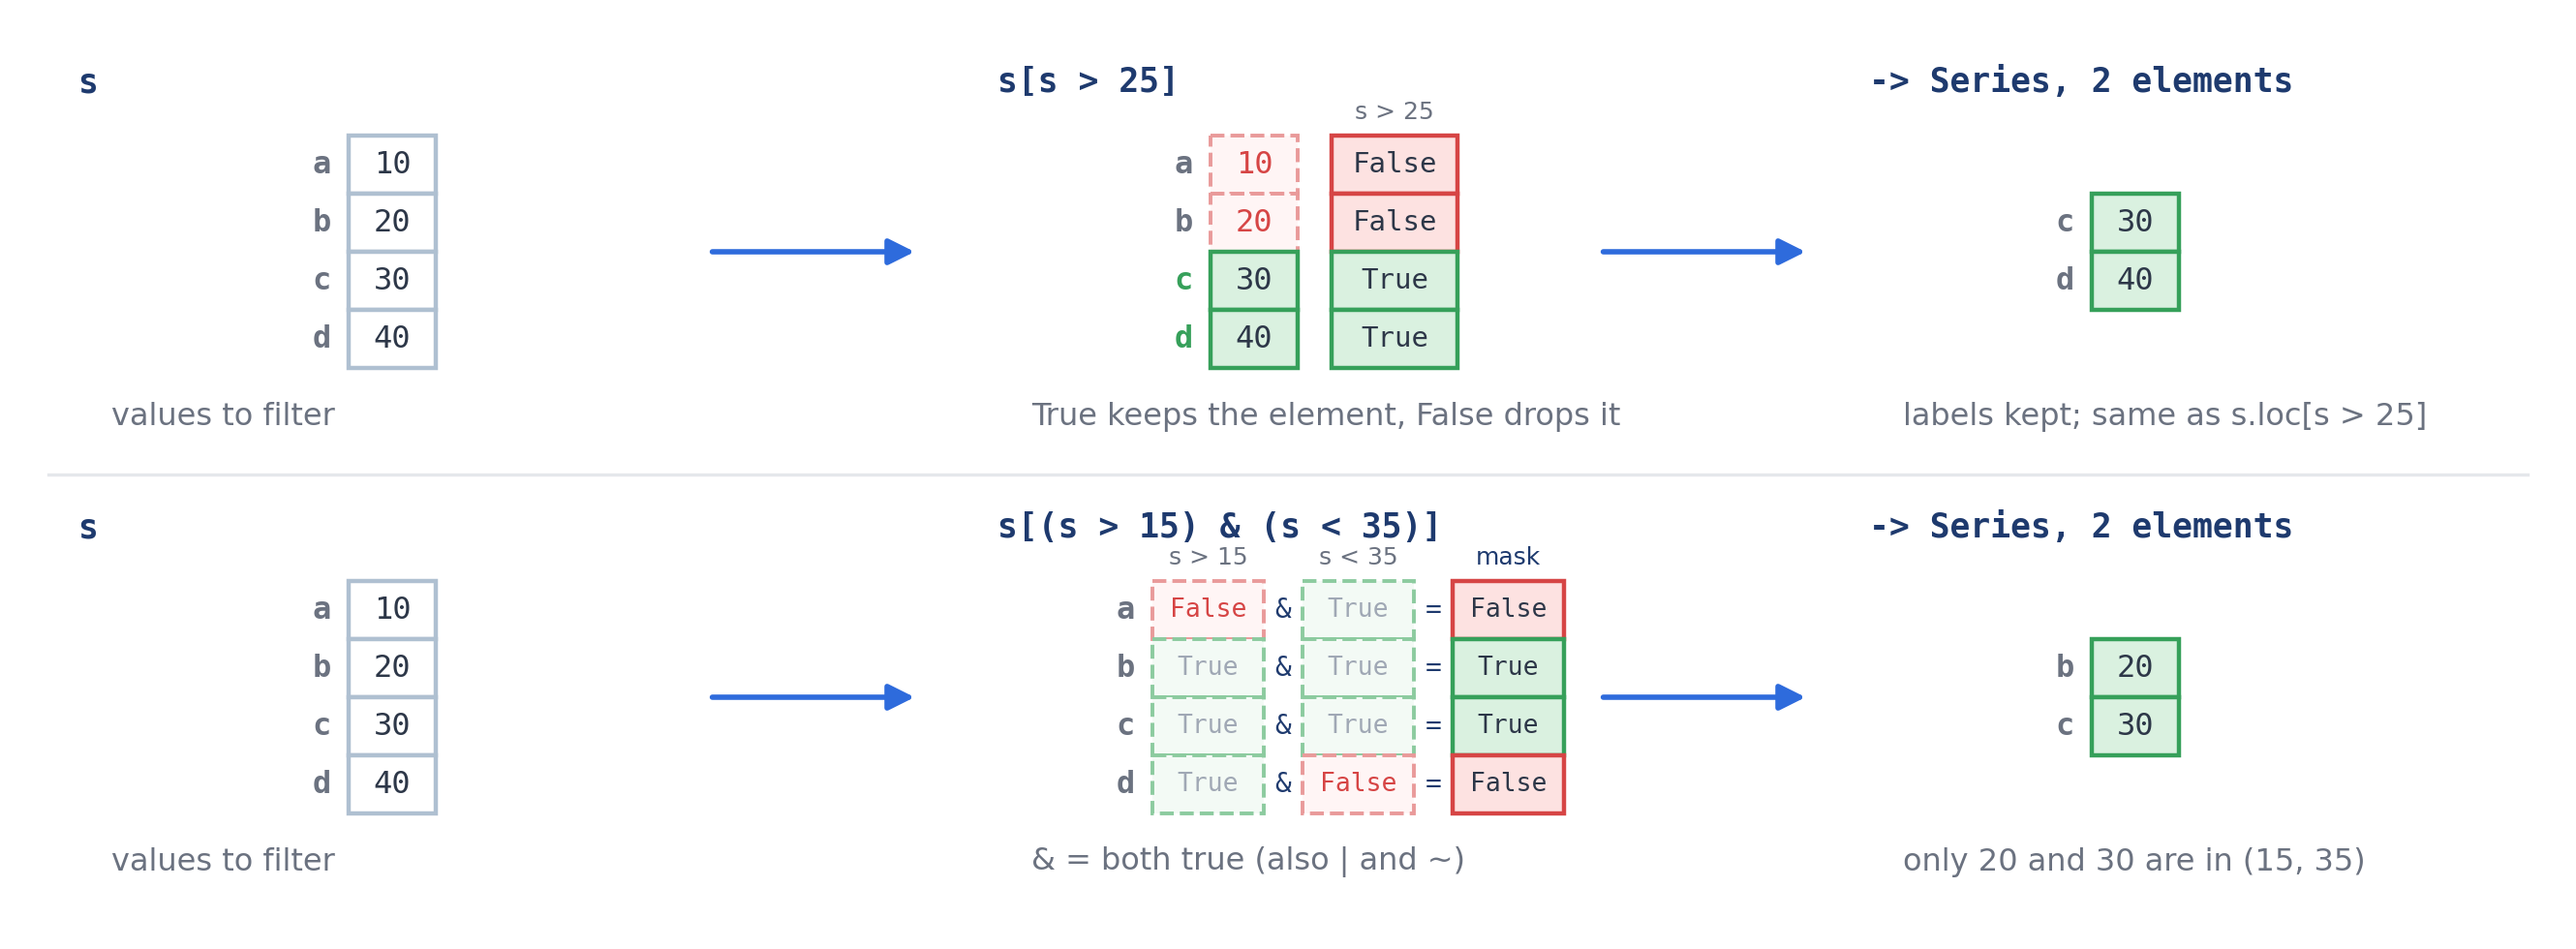
\includegraphics[width=1\textwidth]{contents/images/pandas/sub_masking.png}
            \caption{Boolean masking: a comparison produces a boolean Series with the same index, which keeps only the \texttt{True} elements when passed to \texttt{s[...]} or \texttt{s.loc[...]}. Conditions are combined with \texttt{\&}, \texttt{|}, \texttt{\textasciitilde}; \texttt{.iloc} rejects a boolean Series.}
        \end{figure}
    
    \item \textbf{Fancy Indexing:} You can pass a list of labels to \texttt{.loc} or a list of integer positions to \texttt{.iloc}.
        \begin{figure}[h]
            \centering
            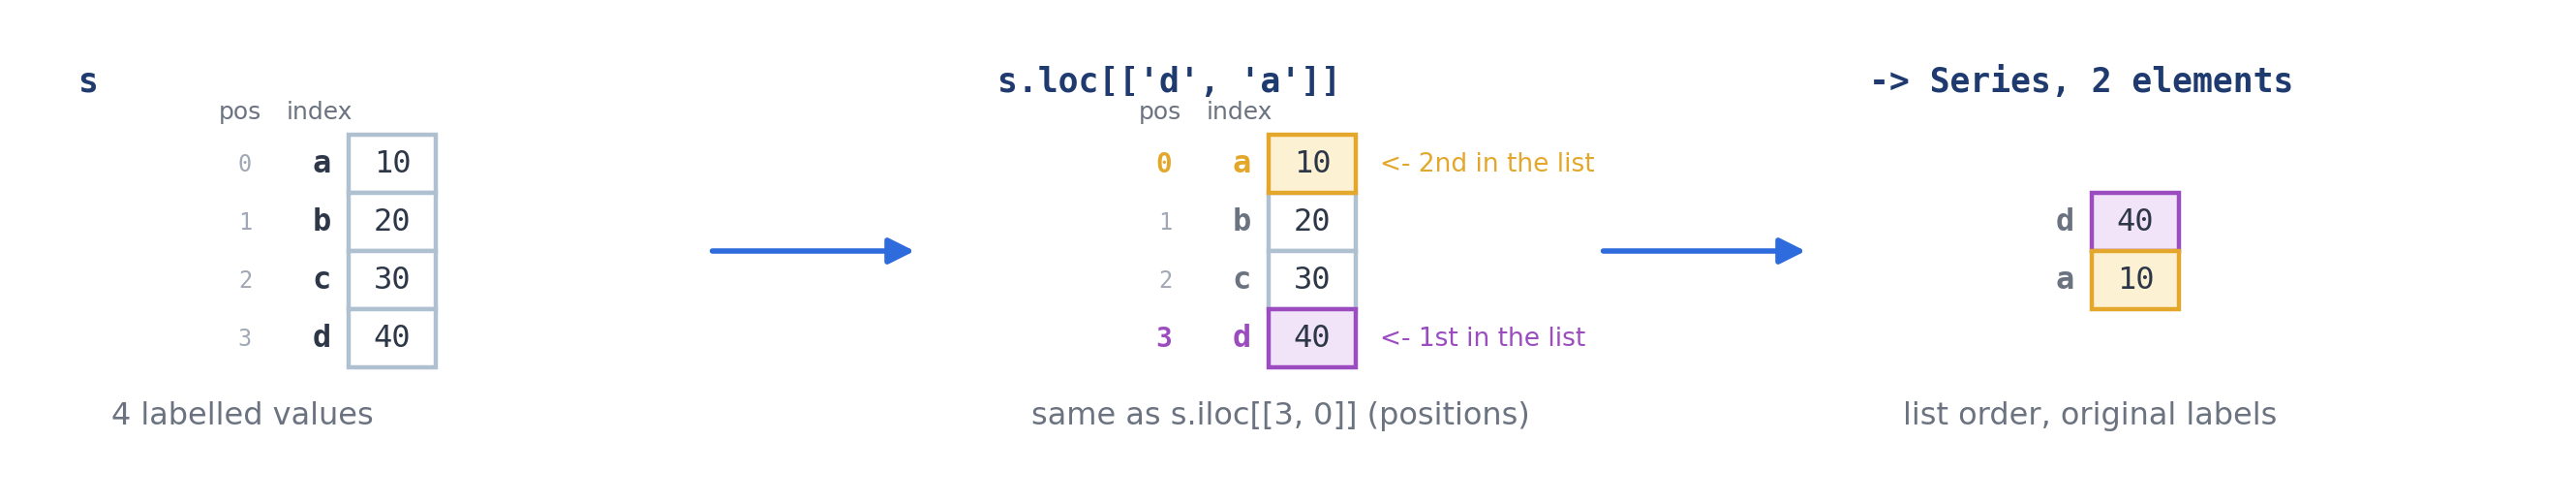
\includegraphics[width=1\textwidth]{contents/images/pandas/sub_fancy_indexing.png}
            \caption{Fancy indexing: a list of labels (\texttt{loc}) or positions (\texttt{iloc}) returns the elements in the order of the list, repetitions included. A label that is not in the index raises a \texttt{KeyError}.}
        \end{figure}

\end{itemize}


\section{DataFrames}

\subsection{A Table of Series}
A DataFrame is a two-dimensional table where each column is an independent Series. While all columns share the same row index, each column maintains its own distinct \texttt{dtype}.

\begin{figure}[h]
    \centering
    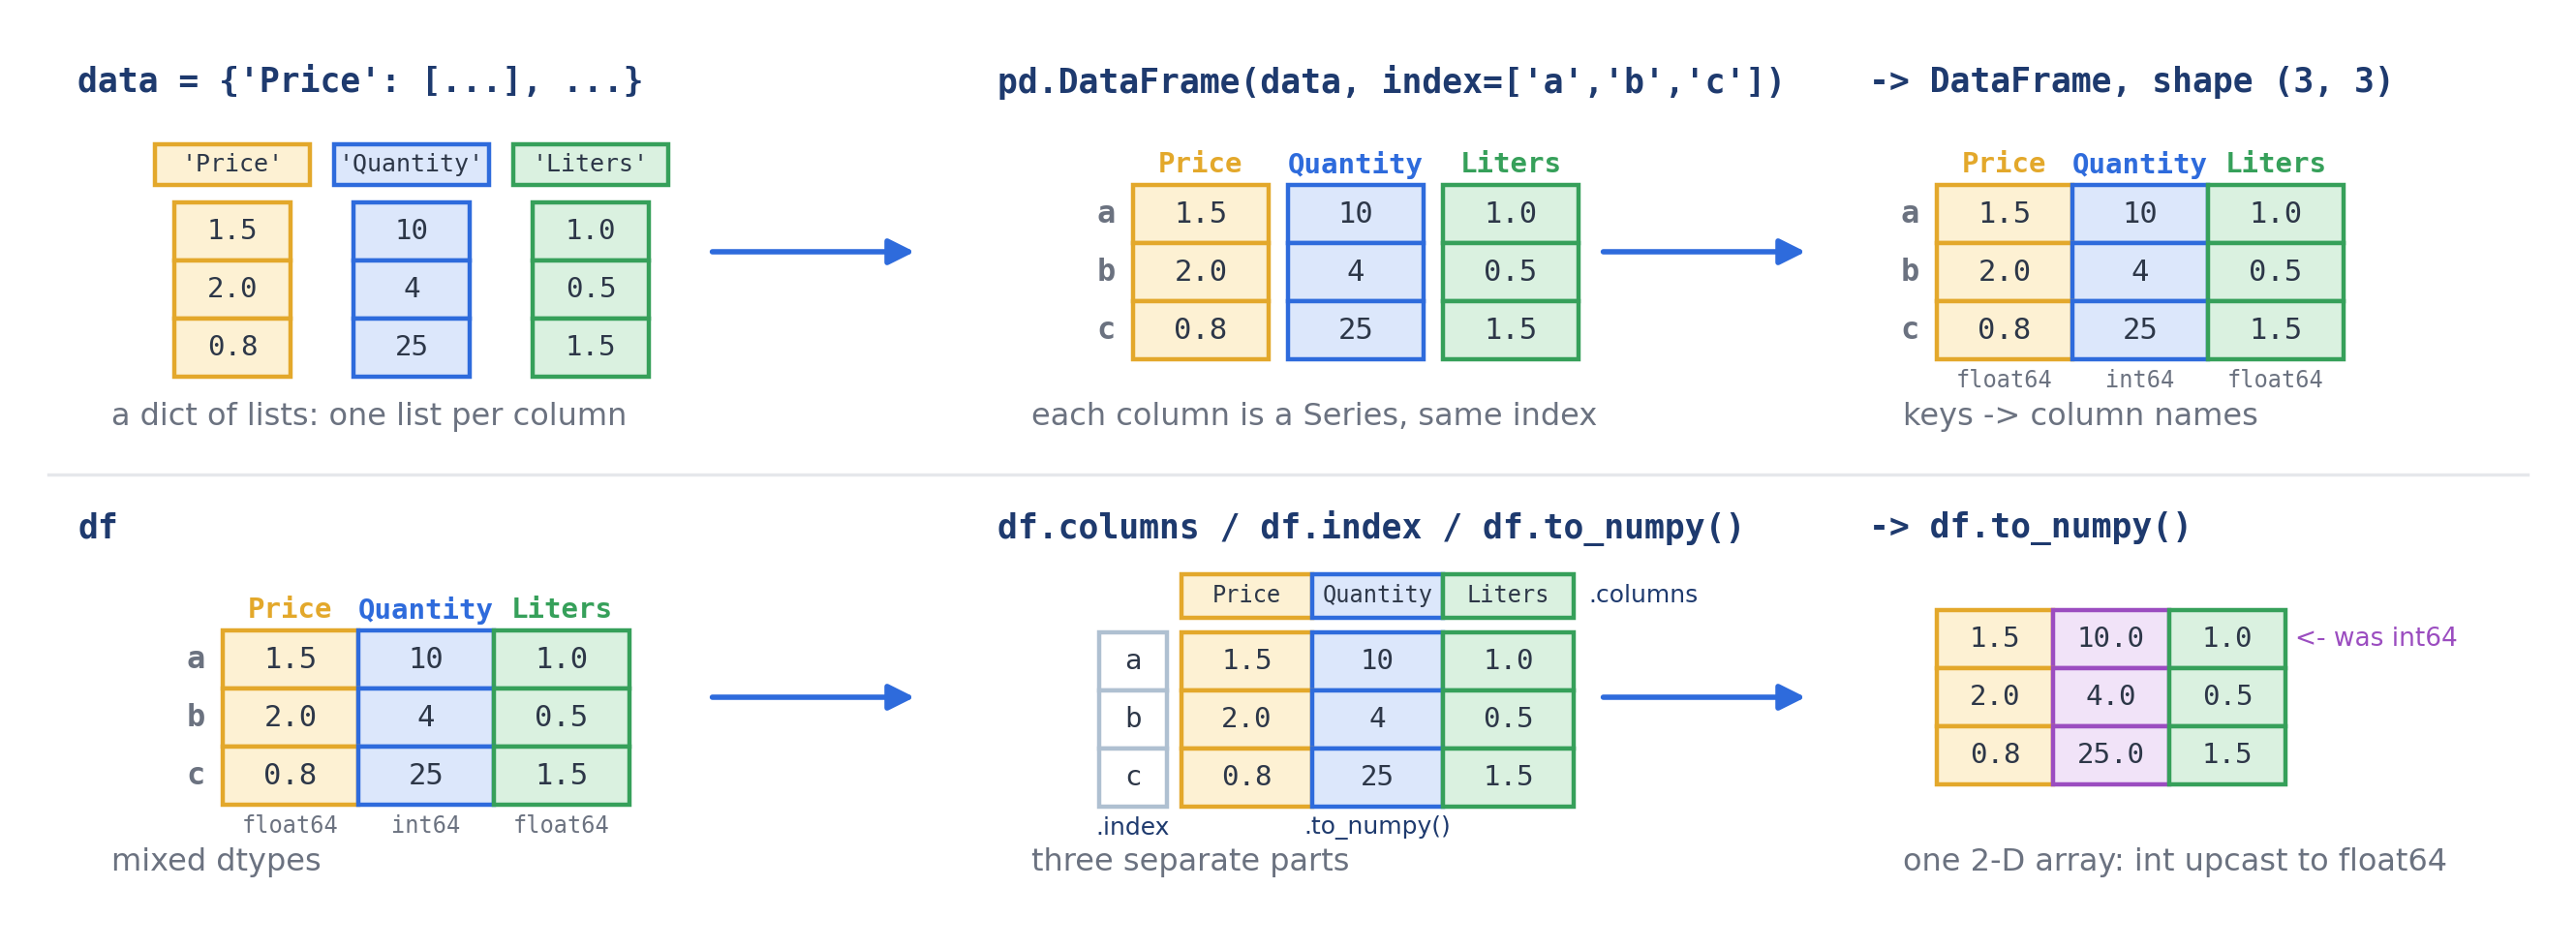
\includegraphics[width=1\textwidth]{contents/images/pandas/sub_dataframe_structure.png}
    \caption{A DataFrame built from a dictionary of lists: each key becomes a column (a Series with its own \texttt{dtype}) and all columns share the same index. \texttt{df.columns}, \texttt{df.index} and \texttt{df.to\_numpy()} return the three parts separately; in the array the \texttt{int64} column is upcast to \texttt{float64}.}
\end{figure}

\begin{itemize}
    \item DataFrames can be created from a dictionary of Series/lists (where keys become column names), a list of dictionaries, or a 2D NumPy array
    \item Core attributes include \texttt{df.columns} (the column names), \texttt{df.index} (the row labels), and \texttt{df.to\_numpy()} (the raw data as a 2D array). When converting to a single NumPy array, pandas upcasts the data to a type capable of holding all columns.
\end{itemize}

\lstinputlisting[caption={Creating and inspecting a DataFrame.}]{contents/listings/pandas/dataframe_creation.py}

\subsection{Accessing Columns and Rows}
On a DataFrame, plain brackets and \texttt{loc}/\texttt{iloc} serve completely different purposes:

\begin{figure}[h]
    \centering
    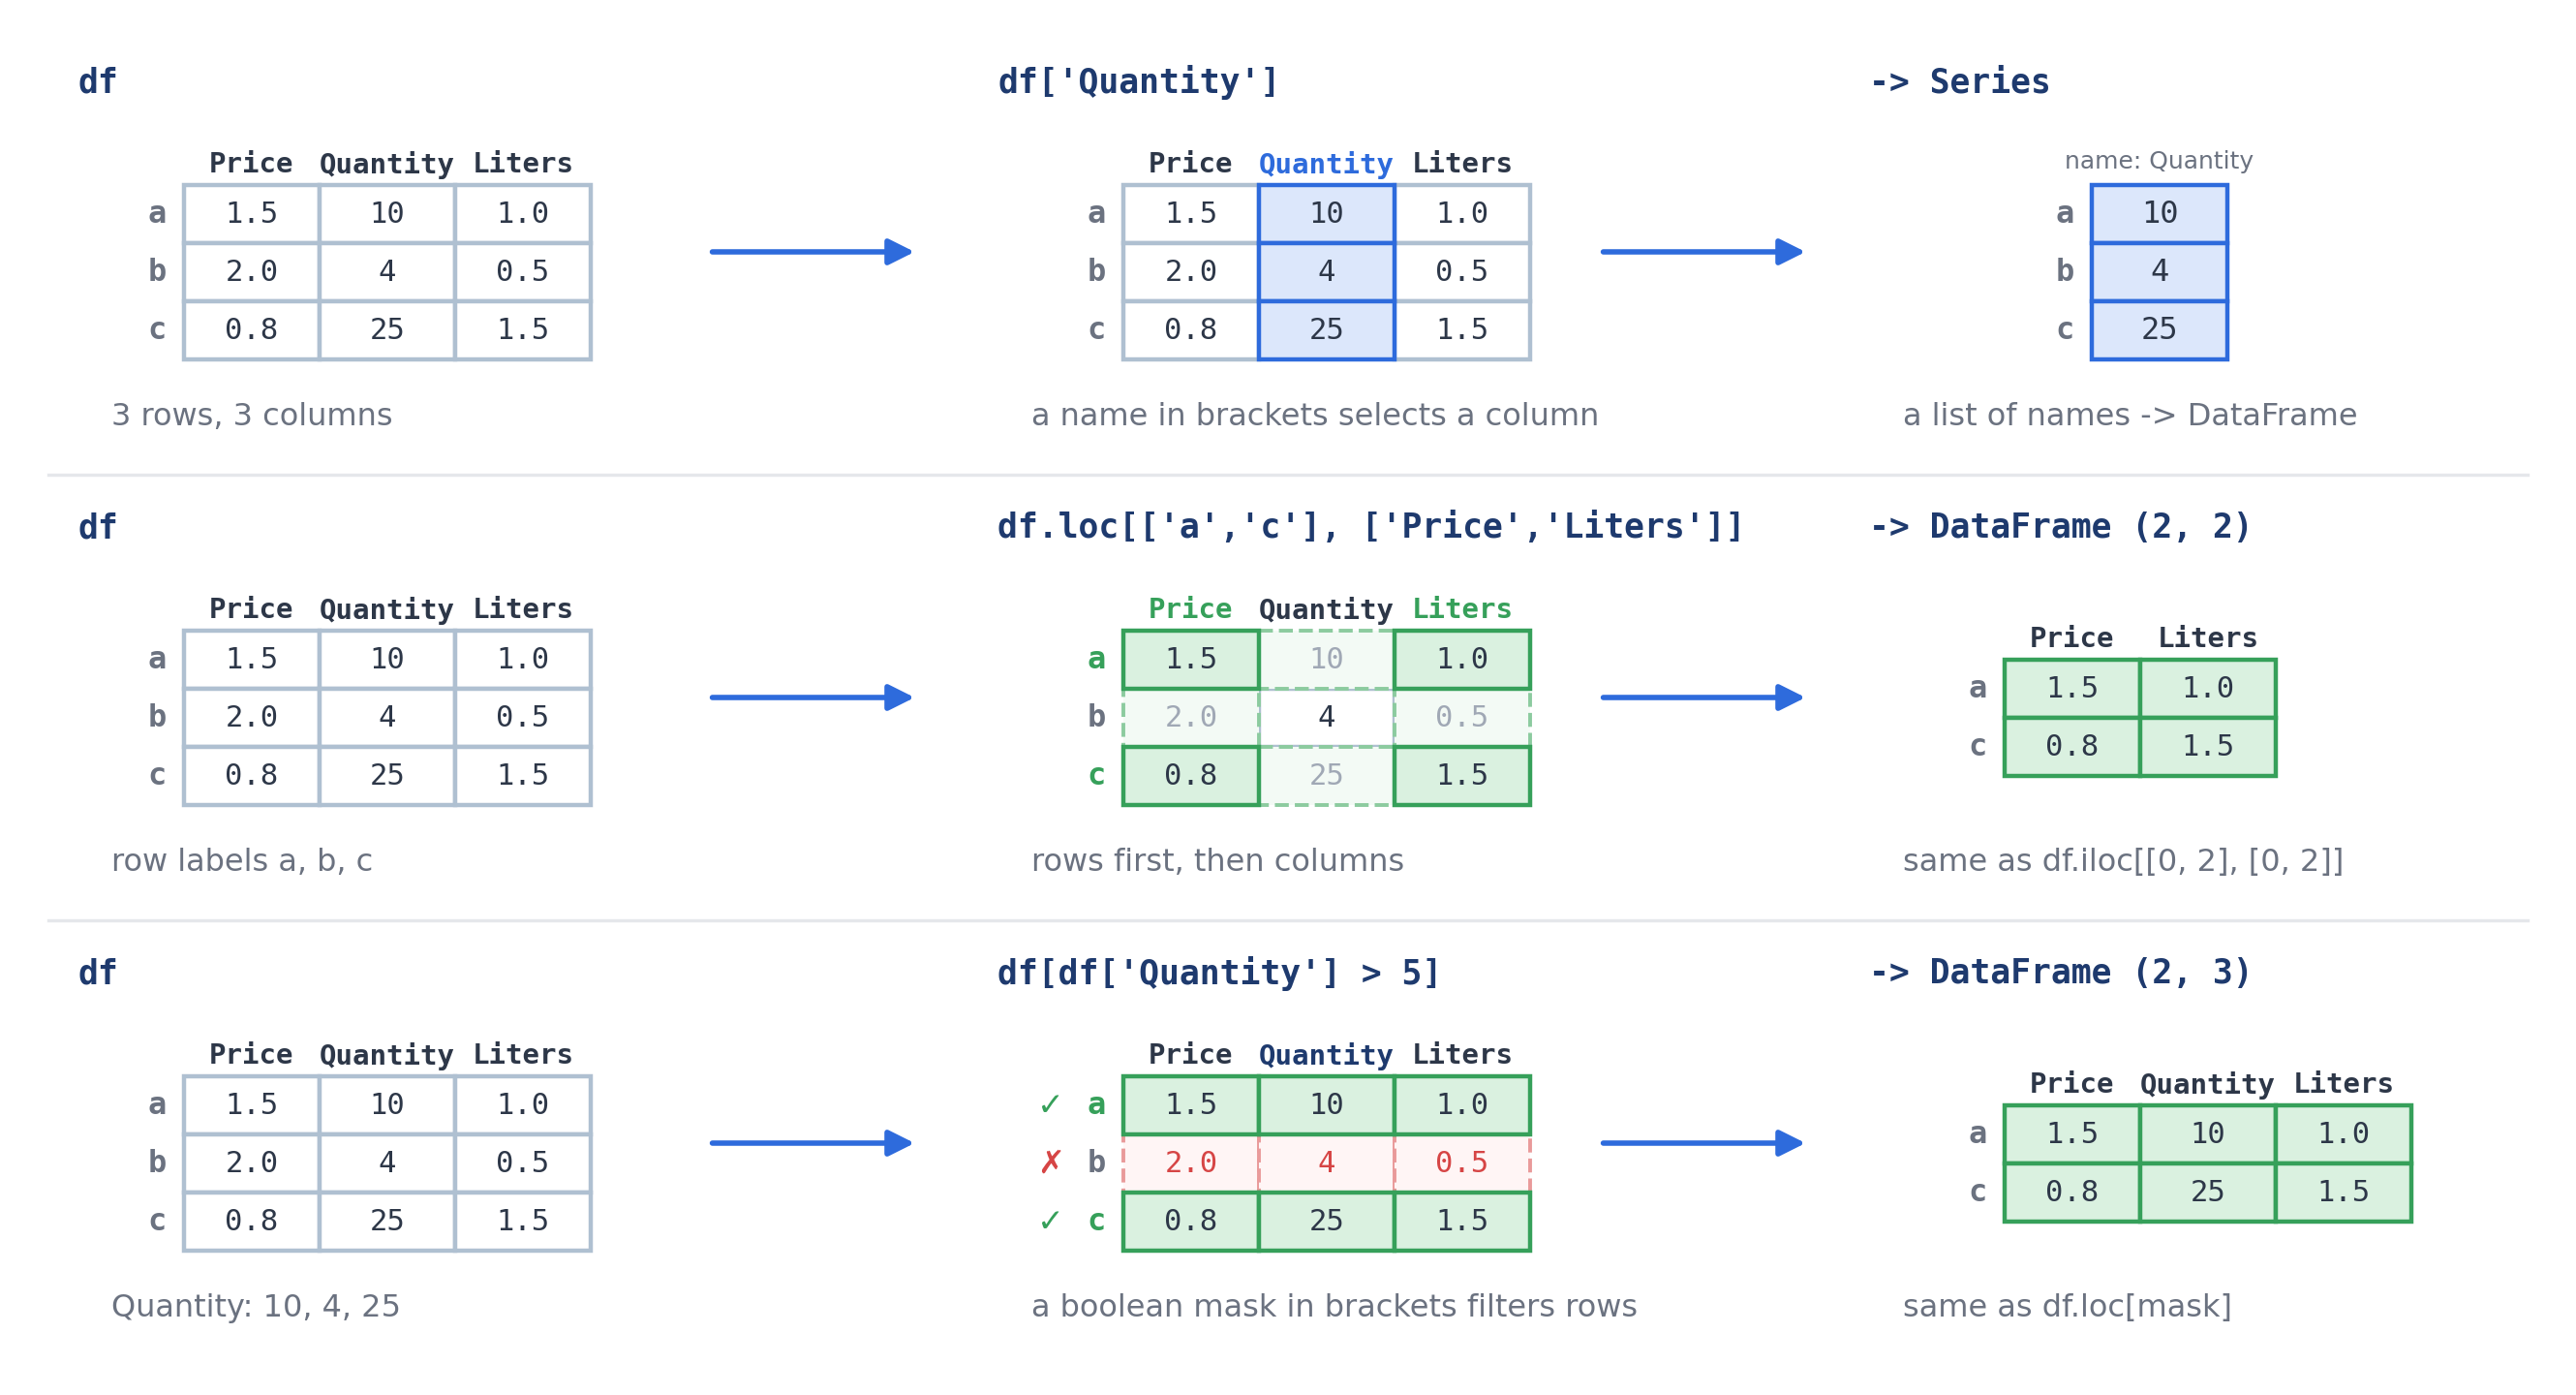
\includegraphics[width=1\textwidth]{contents/images/pandas/sub_dataframe_access.png}
    \caption{Selecting from a DataFrame: a column name in brackets returns a Series, \texttt{df.loc[rows, columns]} returns the intersection of the chosen rows and columns, and a boolean mask in brackets keeps only the rows where it is \texttt{True}.}
\end{figure}

\begin{itemize}
    \item \textbf{Columns:} A name (or list of names) in plain brackets selects columns (\texttt{df['Quantity']} returns a Series, \texttt{df[['Price', 'Liters']]} returns a DataFrame).
    \item \textbf{Rows \& Grids:} \texttt{.loc} and \texttt{.iloc} select rows, or both rows and columns if two selectors are provided (\texttt{df.loc[rows, columns]}).
    \item \textbf{Masking shortcut:} A boolean mask passed directly in plain brackets (e.g., \texttt{df[mask]}) is a ubiquitous shorthand for filtering rows, equivalent to \texttt{df.loc[mask]}.
\end{itemize}

\lstinputlisting[caption={Selecting rows, columns, and applying boolean masks on a DataFrame.}]{contents/listings/pandas/dataframe_access.py}

\subsection{Adding, Modifying, and Copy-on-Write}
You can add or replace columns by assigning them to a name (\texttt{df["NewCol"] = ...}). Methods like \texttt{rename} and \texttt{drop} return a new DataFrame without altering the original.

\begin{figure}[h]
    \centering
    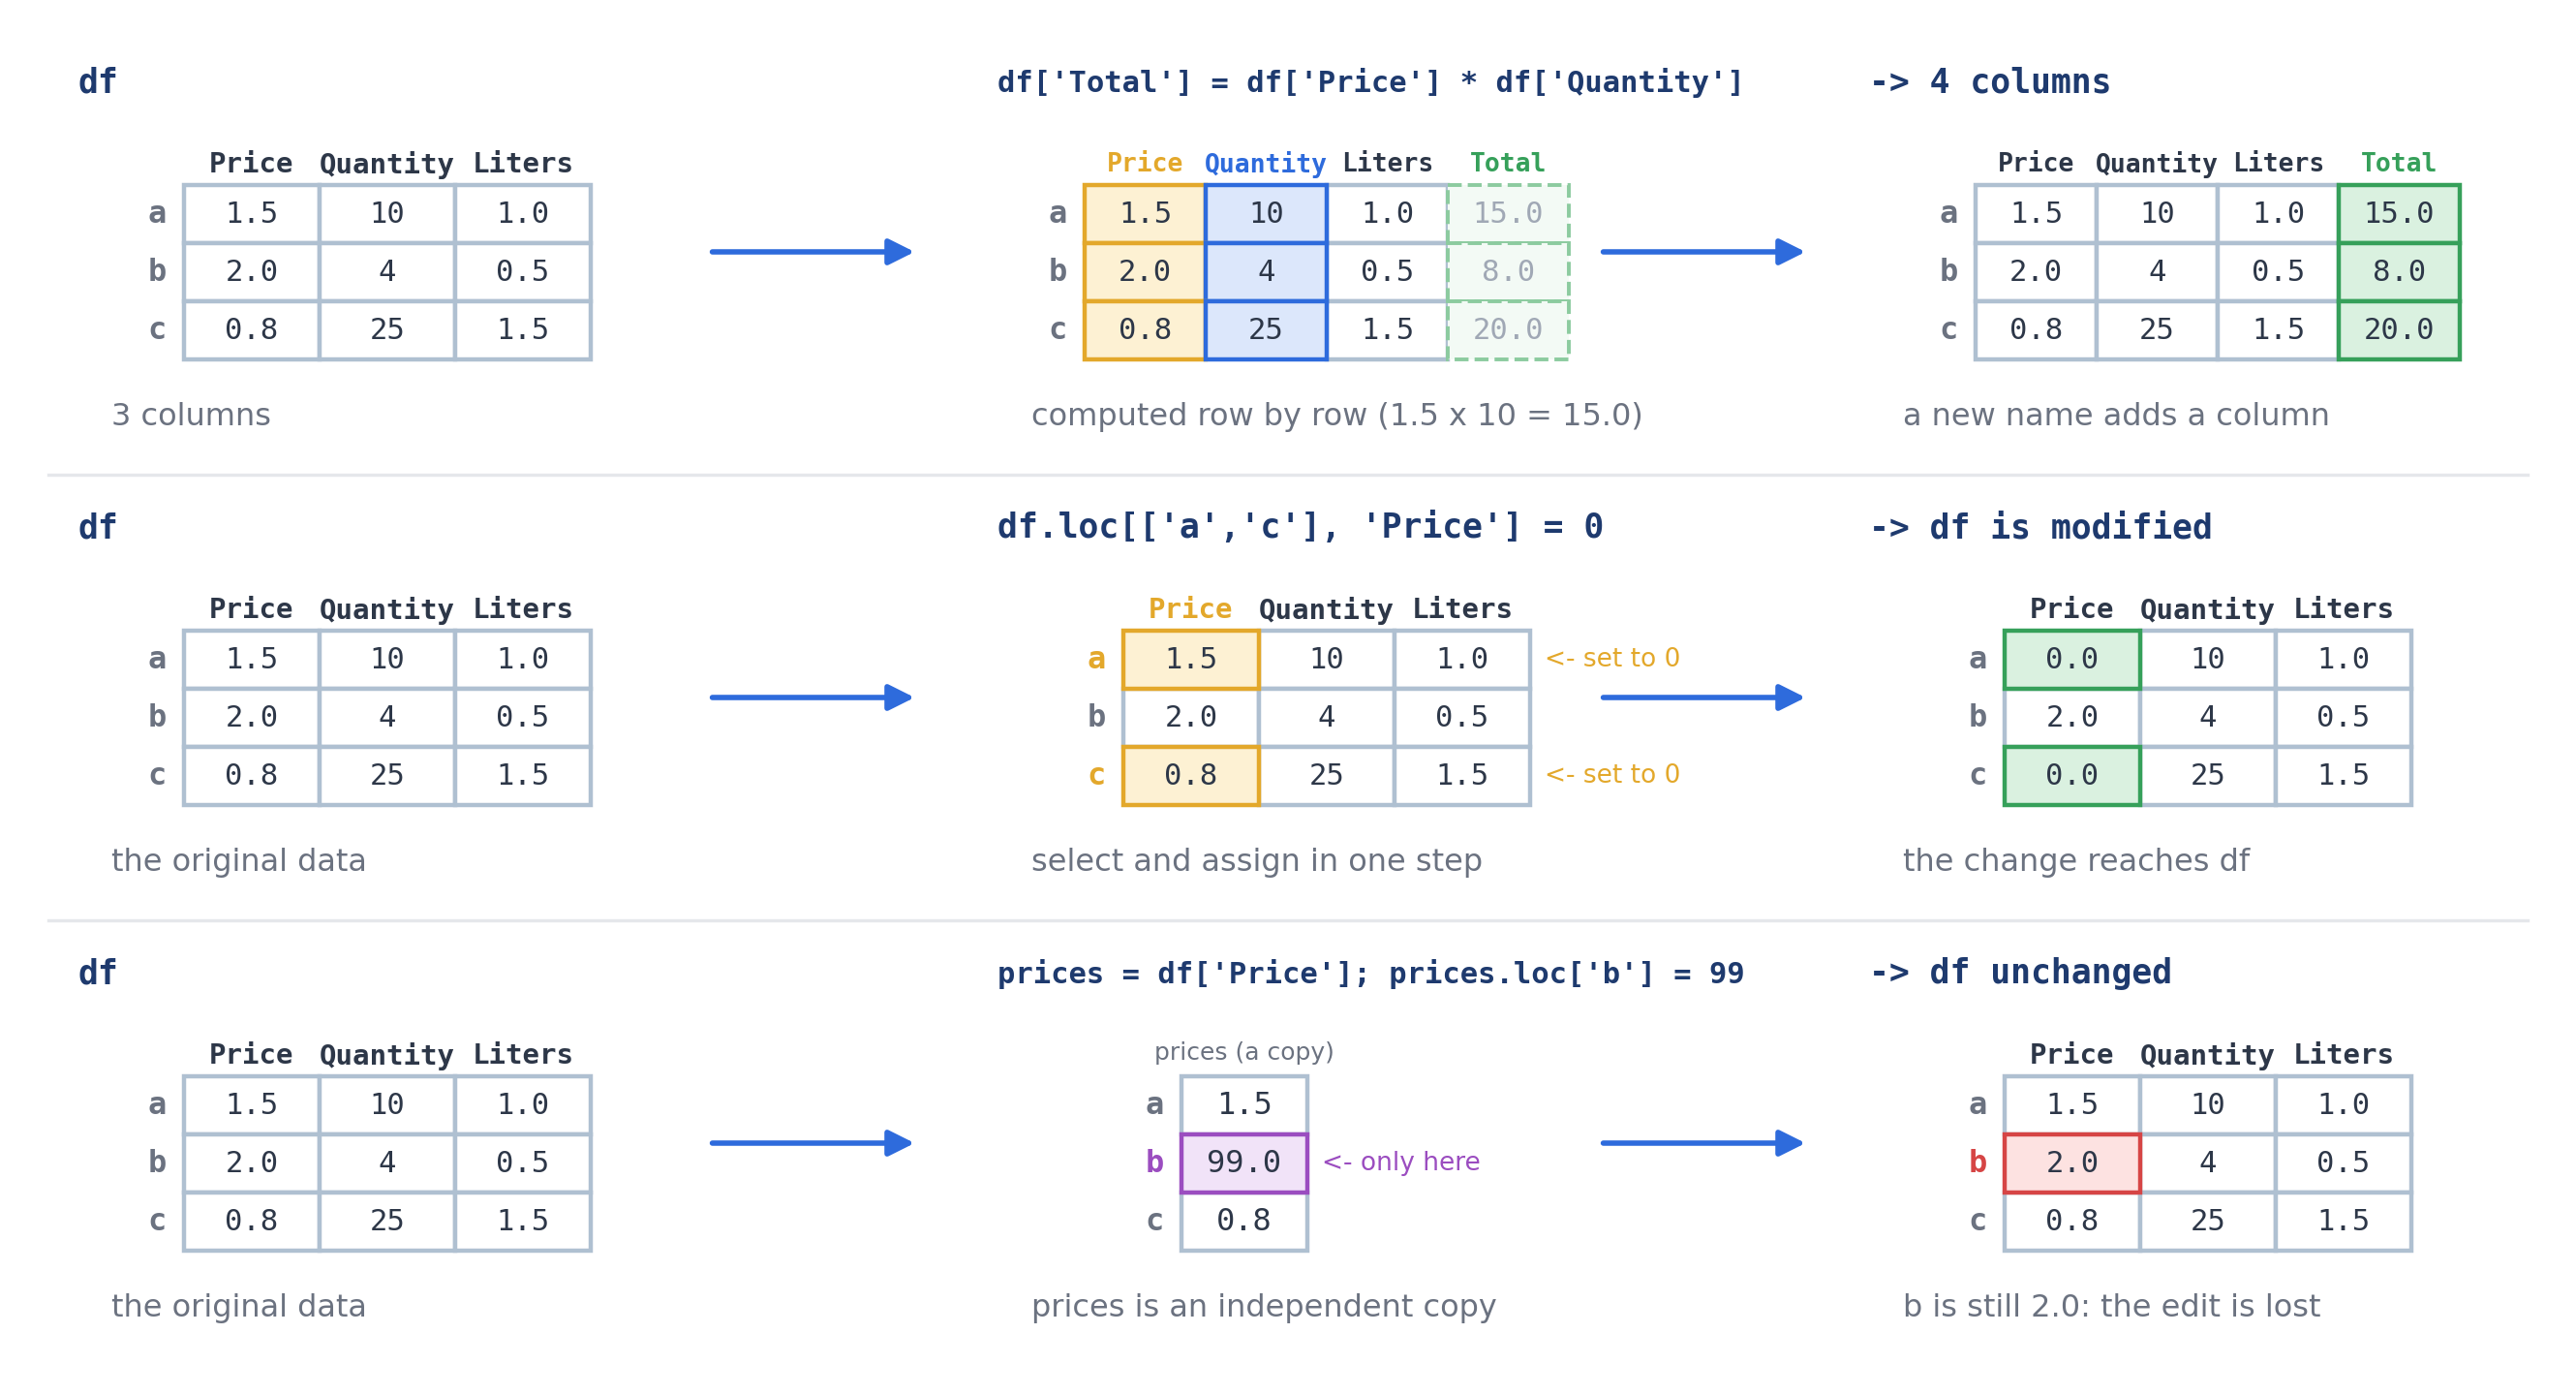
\includegraphics[width=1\textwidth]{contents/images/pandas/sub_dataframe_modify.png}
    \caption{Modifying a DataFrame: assigning to a new name adds a column; \texttt{df.loc[rows, column] = value} changes \texttt{df} in a single step; with Copy-on-Write, an edit made through an intermediate variable changes only the copy and is lost for \texttt{df}.}
\end{figure}

\textbf{Copy-on-Write (pandas 3.0+):}
Any piece of data extracted from a DataFrame (a column, slice, or mask) behaves as an independent copy. To safely modify the original DataFrame, you must perform the selection and assignment in a single operation:
\begin{itemize}
    \item \textbf{Correct:} \texttt{df.loc[["a", "c"], "Price"] = 0} (modifies \texttt{df} directly).
    \item \textbf{Incorrect:} \texttt{prices = df["Price"]; prices.loc["b"] = 99} (modifies the copy, leaving \texttt{df} unchanged).
\end{itemize}

\lstinputlisting[caption={Adding columns and assigning values properly.}]{contents/listings/pandas/dataframe_modify.py}



\section{Computation with pandas}
Pandas supports three main types of computational operations: unary operations, aggregations, and operations between pandas objects.

\subsection{Unary Operations}
Unary operations are applied element-by-element. You can perform standard arithmetic (e.g., \texttt{s / 4 + 1}) or apply NumPy universal functions (e.g., \texttt{np.abs(s)}) directly to a Series or DataFrame. The resulting object retains the exact same index and labels as the original.

\begin{figure}[h]
    \centering
    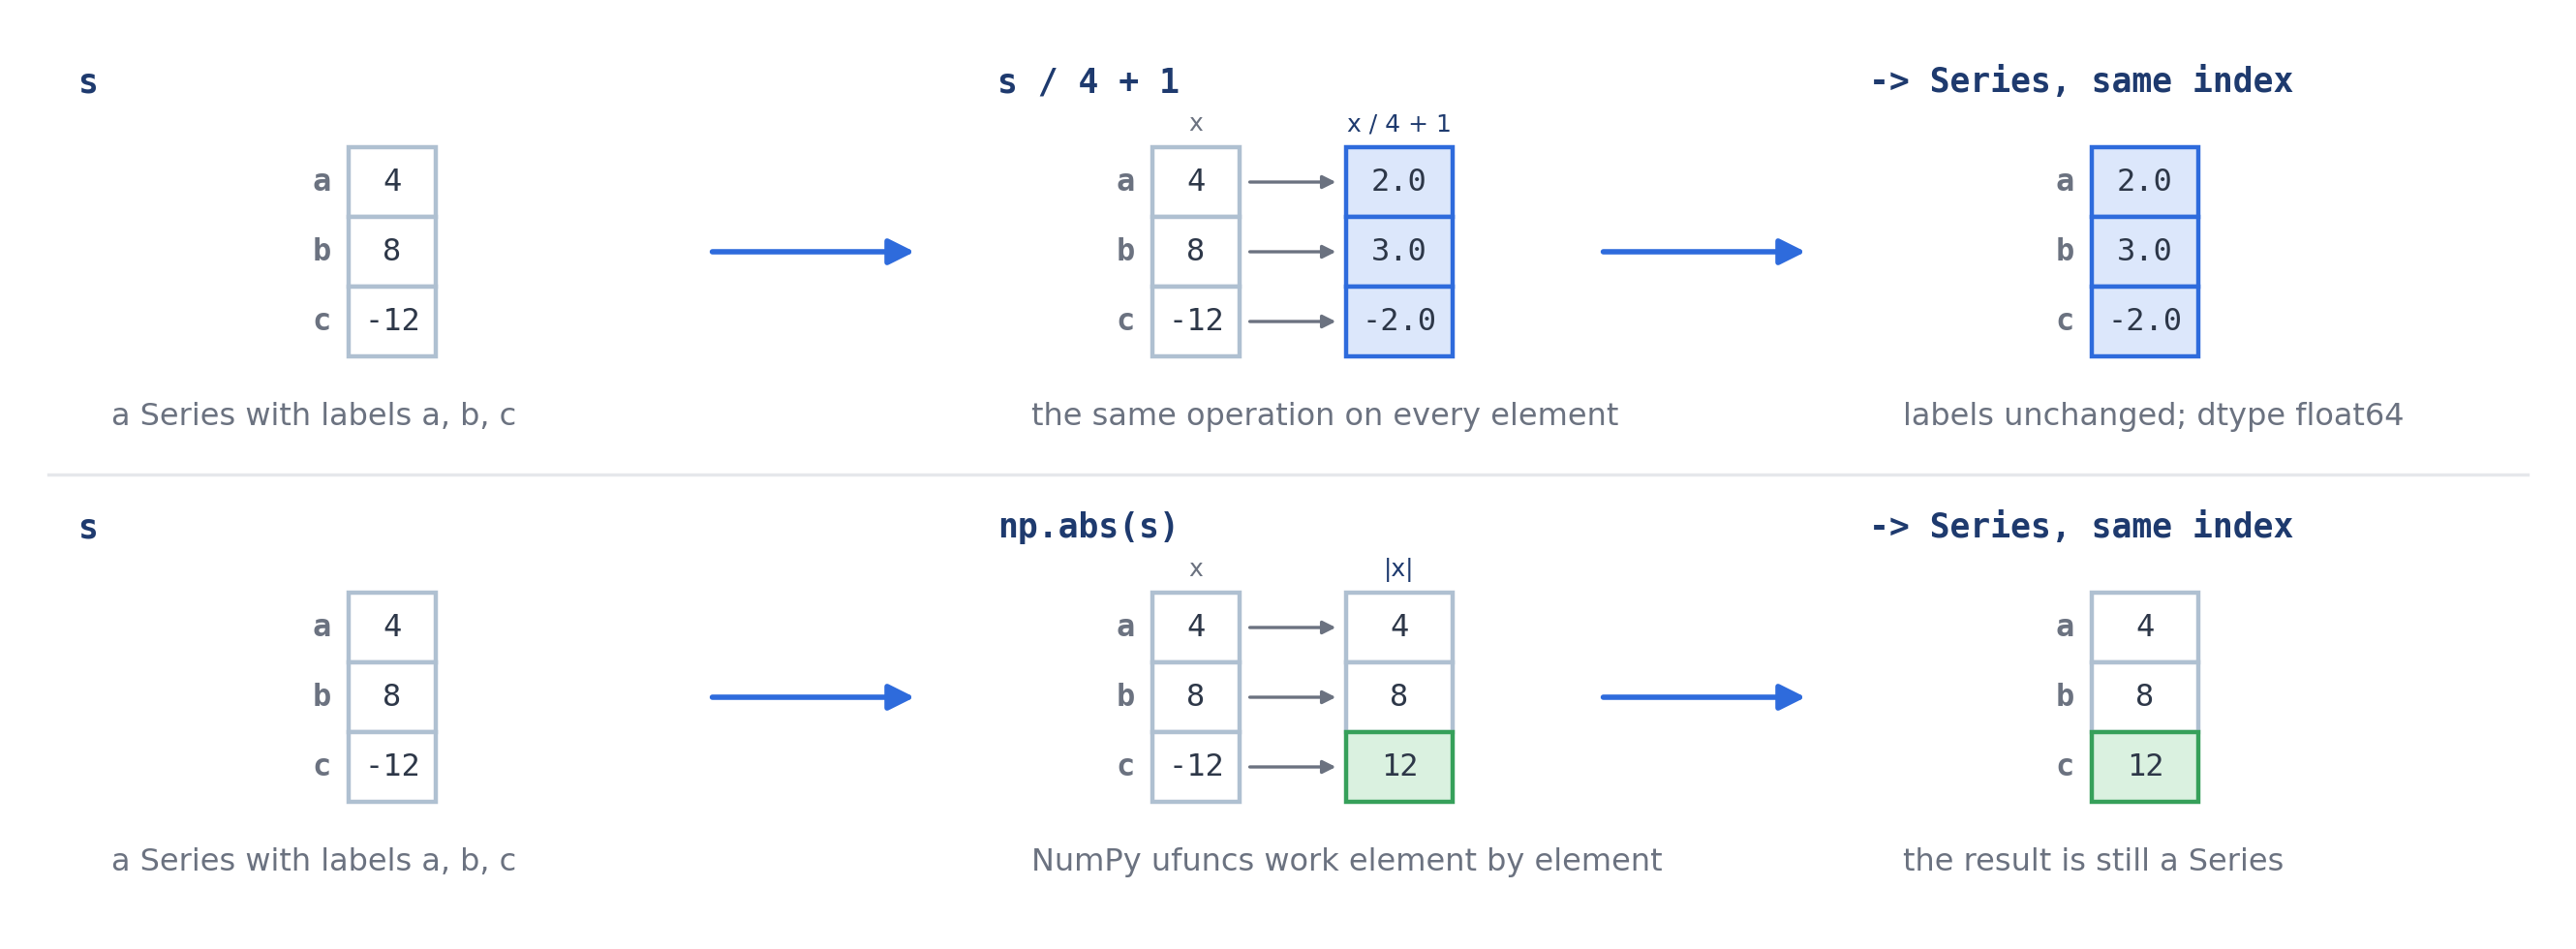
\includegraphics[width=1\textwidth]{contents/images/pandas/sub_unary.png}
    \caption{Unary operations: arithmetic expressions such as \texttt{s / 4 + 1} and NumPy ufuncs such as \texttt{np.abs(s)} are applied to every element, and the result keeps the original index.}
\end{figure}

\lstinputlisting[caption={Applying arithmetic and NumPy ufuncs to a Series.}]{contents/listings/pandas/pandas_unary.py}

\subsection{Operations Between Objects: Alignment}
When performing binary operations (like \texttt{+}, \texttt{-}, \texttt{*}, \texttt{/}) between Series or DataFrames, pandas pairs the elements \textbf{by label, not by position}.

\begin{figure}[h]
    \centering
    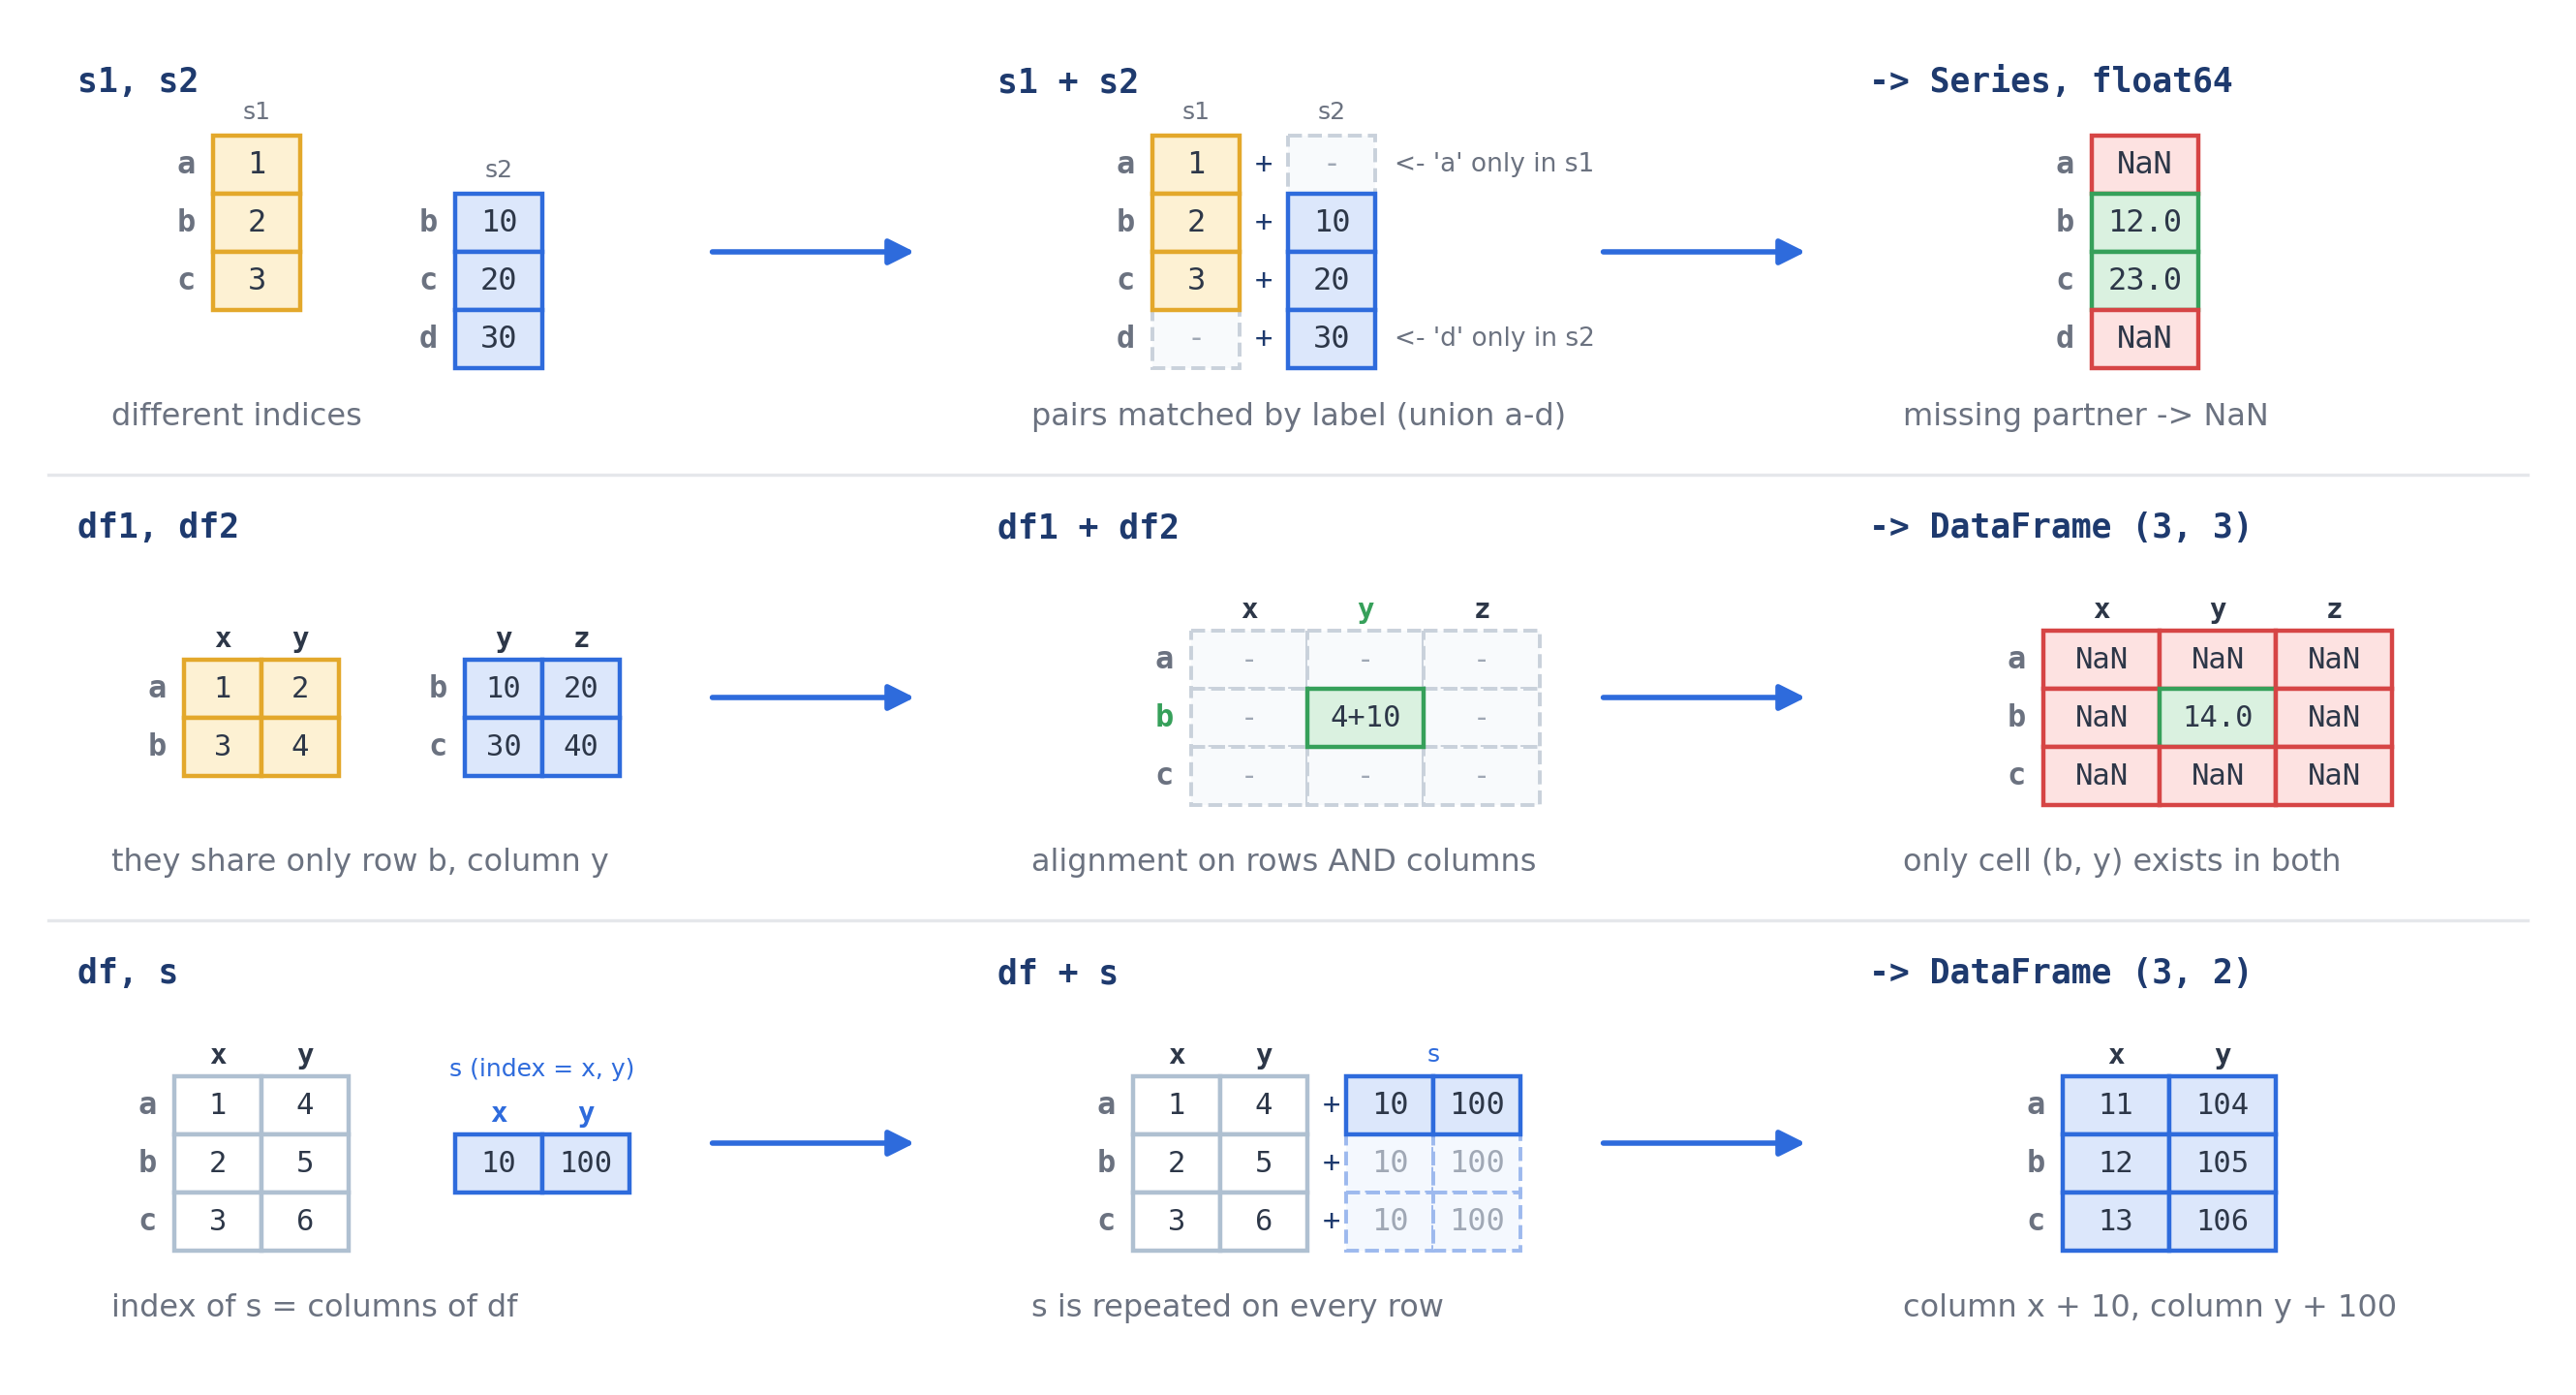
\includegraphics[width=1\textwidth]{contents/images/pandas/sub_alignment.png}
    \caption{Label alignment: two Series are matched by label over the union of their indices, and a label missing on one side gives \texttt{NaN}. Two DataFrames are aligned on both rows and columns. A Series added to a DataFrame is matched to its columns and broadcast over every row.}
\end{figure}

\begin{itemize}
    \item \textbf{Series + Series:} pandas aligns the two Series based on their indices. If a label exists in one Series but not the other, the result for that label is \texttt{NaN} (Not a Number). The final index is the sorted union of both indices. Because \texttt{NaN} is a floating-point value, introducing it will upcast an integer array to \texttt{float64}.
    \item \textbf{DataFrame + DataFrame:} Alignment happens on both axes (rows and columns). A cell only computes a valid result if both its row label and column label exist in both DataFrames; otherwise, it becomes \texttt{NaN}.
    \item \textbf{Broadcasting (DataFrame + Series):} When operating between a DataFrame and a Series, pandas matches the index of the Series to the \textbf{columns} of the DataFrame. The Series is then broadcast (repeated) across every row of the DataFrame. 
\end{itemize}

\lstinputlisting[caption={Automatic label alignment and broadcasting.}]{contents/listings/pandas/pandas_alignment.py}

\subsection{Aggregations and Normalization}
Aggregation functions (such as \texttt{mean}, \texttt{std}, \texttt{min}, \texttt{max}, \texttt{sum}) reduce the data.

\begin{figure}[h]
    \centering
    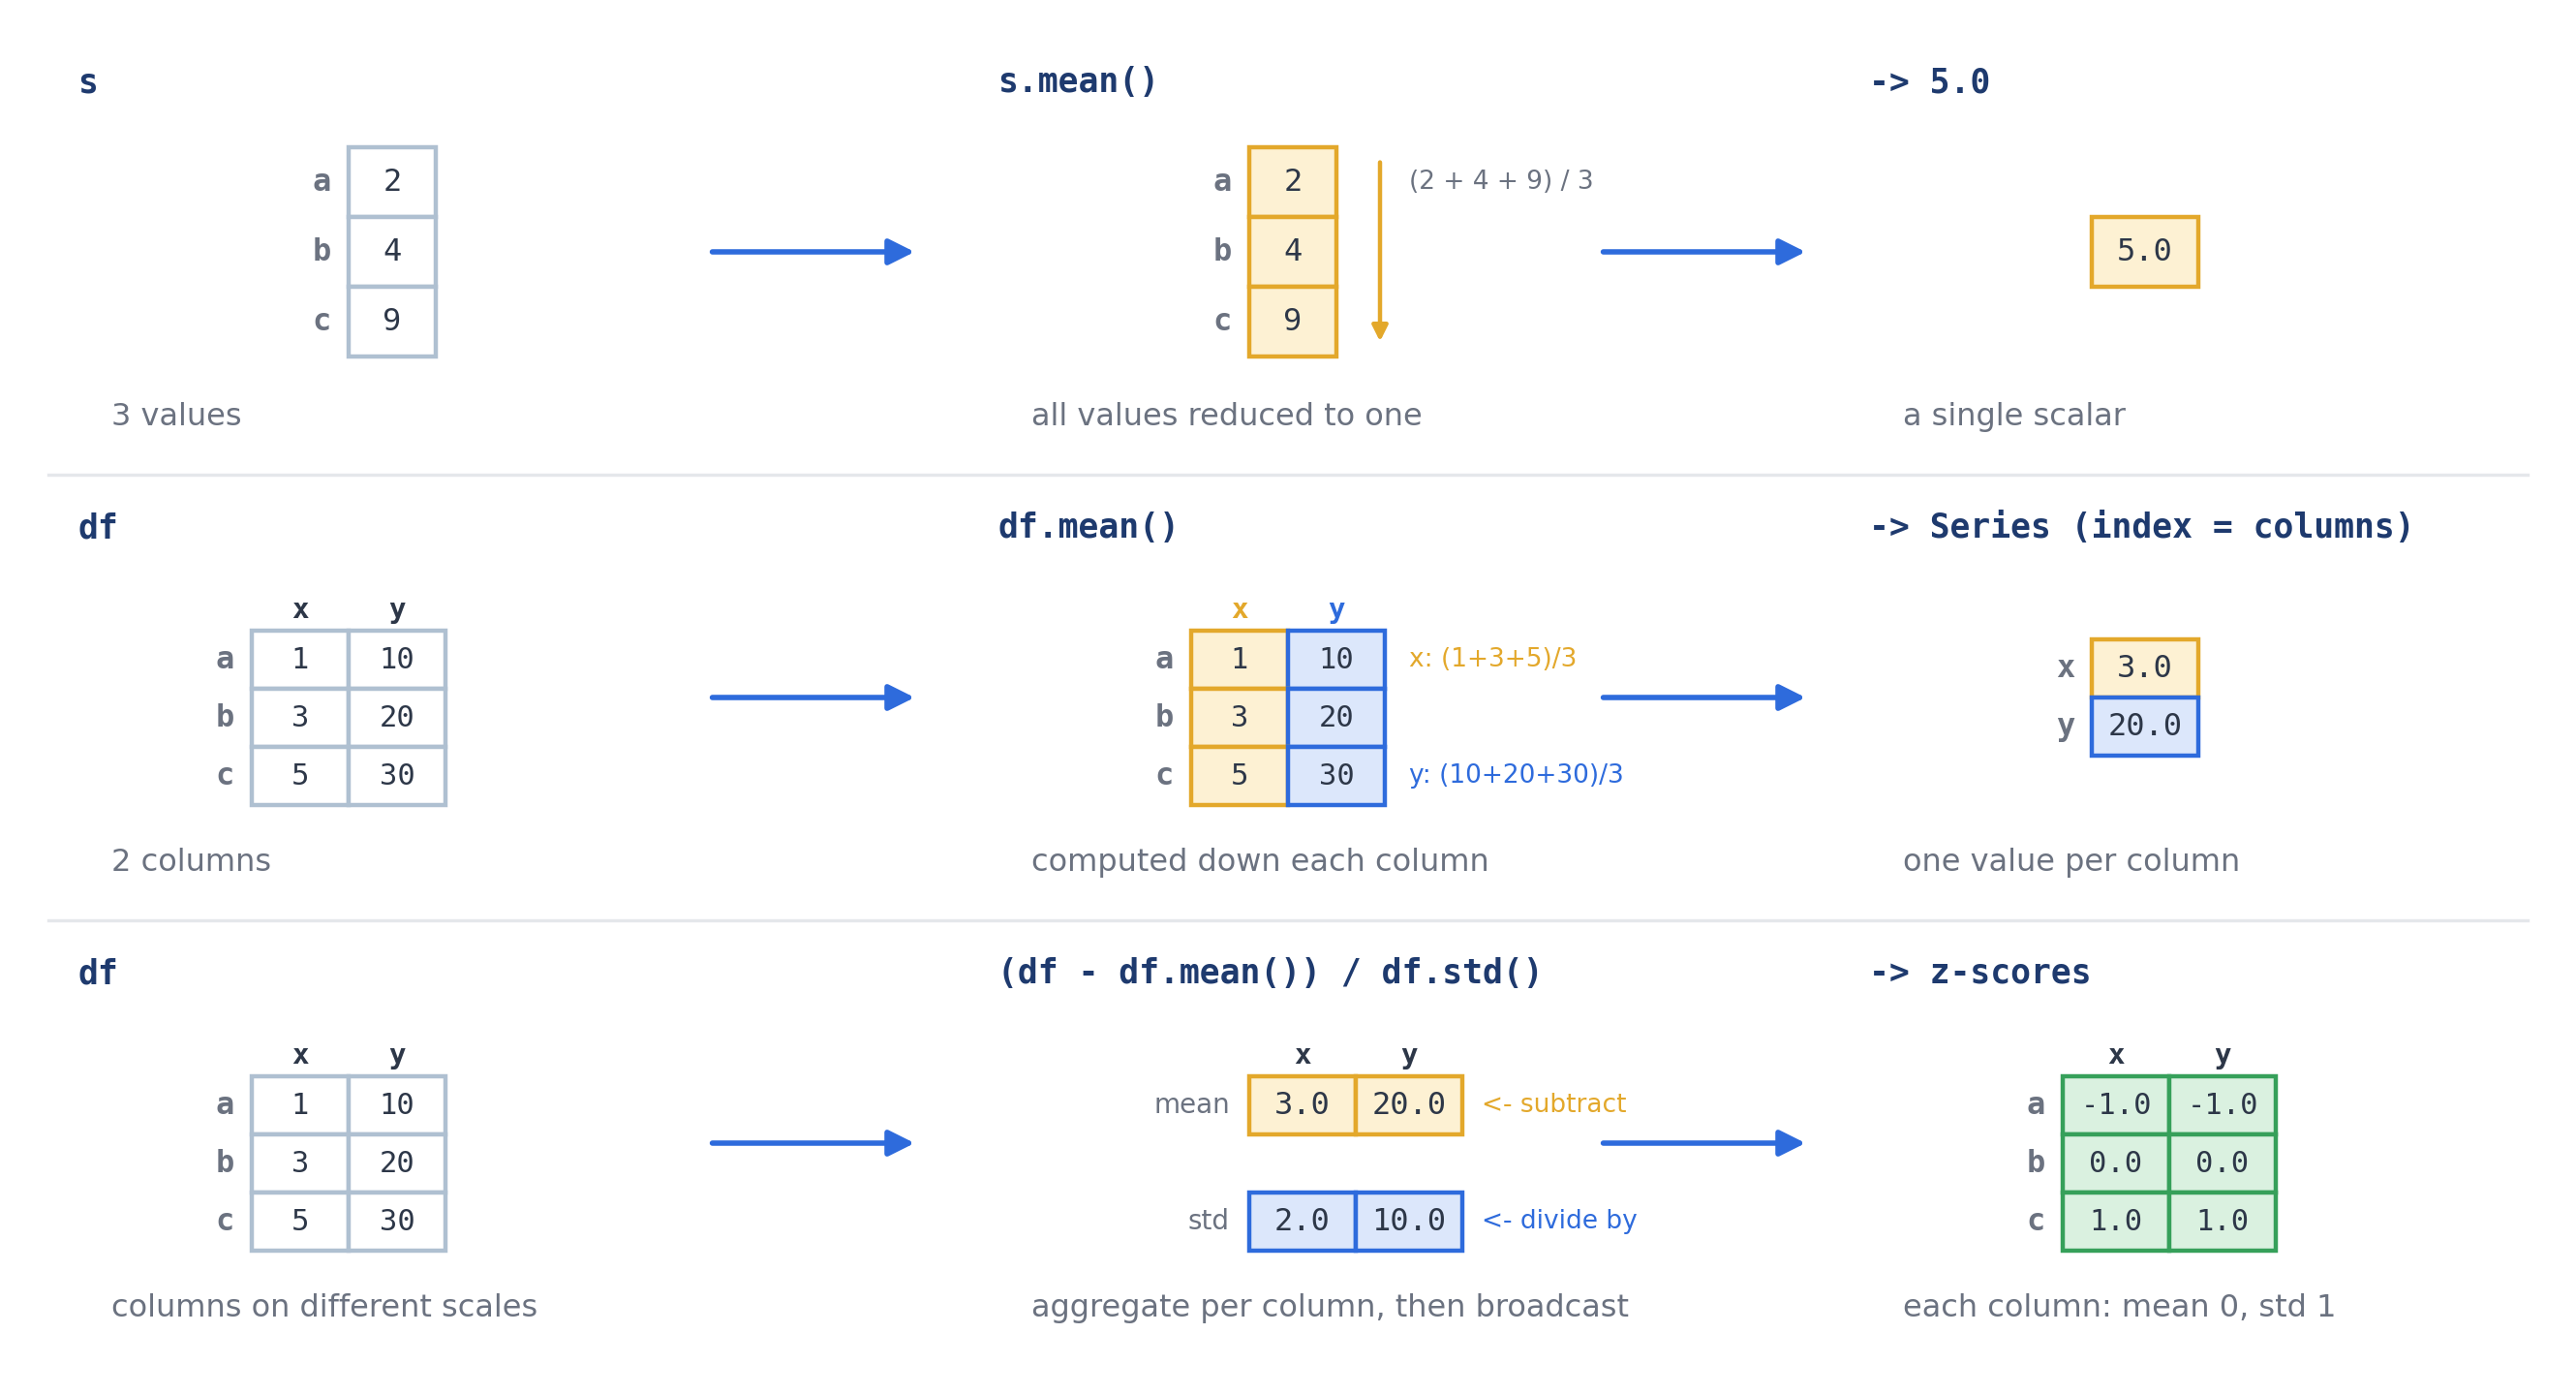
\includegraphics[width=1\textwidth]{contents/images/pandas/sub_aggregations.png}
    \caption{Aggregations: on a Series \texttt{mean()} returns a scalar, on a DataFrame it returns a Series with one value per column. Z-score normalization combines column-wise aggregation and broadcasting: each column ends up with mean 0 and standard deviation 1 (sample \texttt{std}, $\mathrm{ddof}=1$).}
\end{figure}

\begin{itemize}
    \item On a \textbf{Series}, an aggregation returns a single scalar value.
    \item On a \textbf{DataFrame}, the aggregation is computed column by column (iterating over the rows), returning a Series with one value per column.
    \item \textbf{Standard Deviation Note:} By default, \texttt{df.std()} calculates the sample standard deviation (dividing by $n-1$), which differs from NumPy's \texttt{np.std()} (which divides by $n$). To match NumPy's behavior, use \texttt{df.std(ddof=0)}.
\end{itemize}

A common data preprocessing task is Z-score normalization, which leverages both column-wise aggregation and broadcasting to execute without a single loop[cite: 142].

\lstinputlisting[caption={Aggregating DataFrames and Z-score normalization.}]{contents/listings/pandas/pandas_aggregations.py}



\section{Combining Series and DataFrames}
pandas provides two primary functions for putting DataFrames and Series together: \texttt{pd.concat} for stacking them, and \texttt{pd.merge} for joining them based on common values.

\subsection{Concatenation}
The \texttt{pd.concat} function stacks objects (vertically by default). 

\begin{figure}[h]
    \centering
    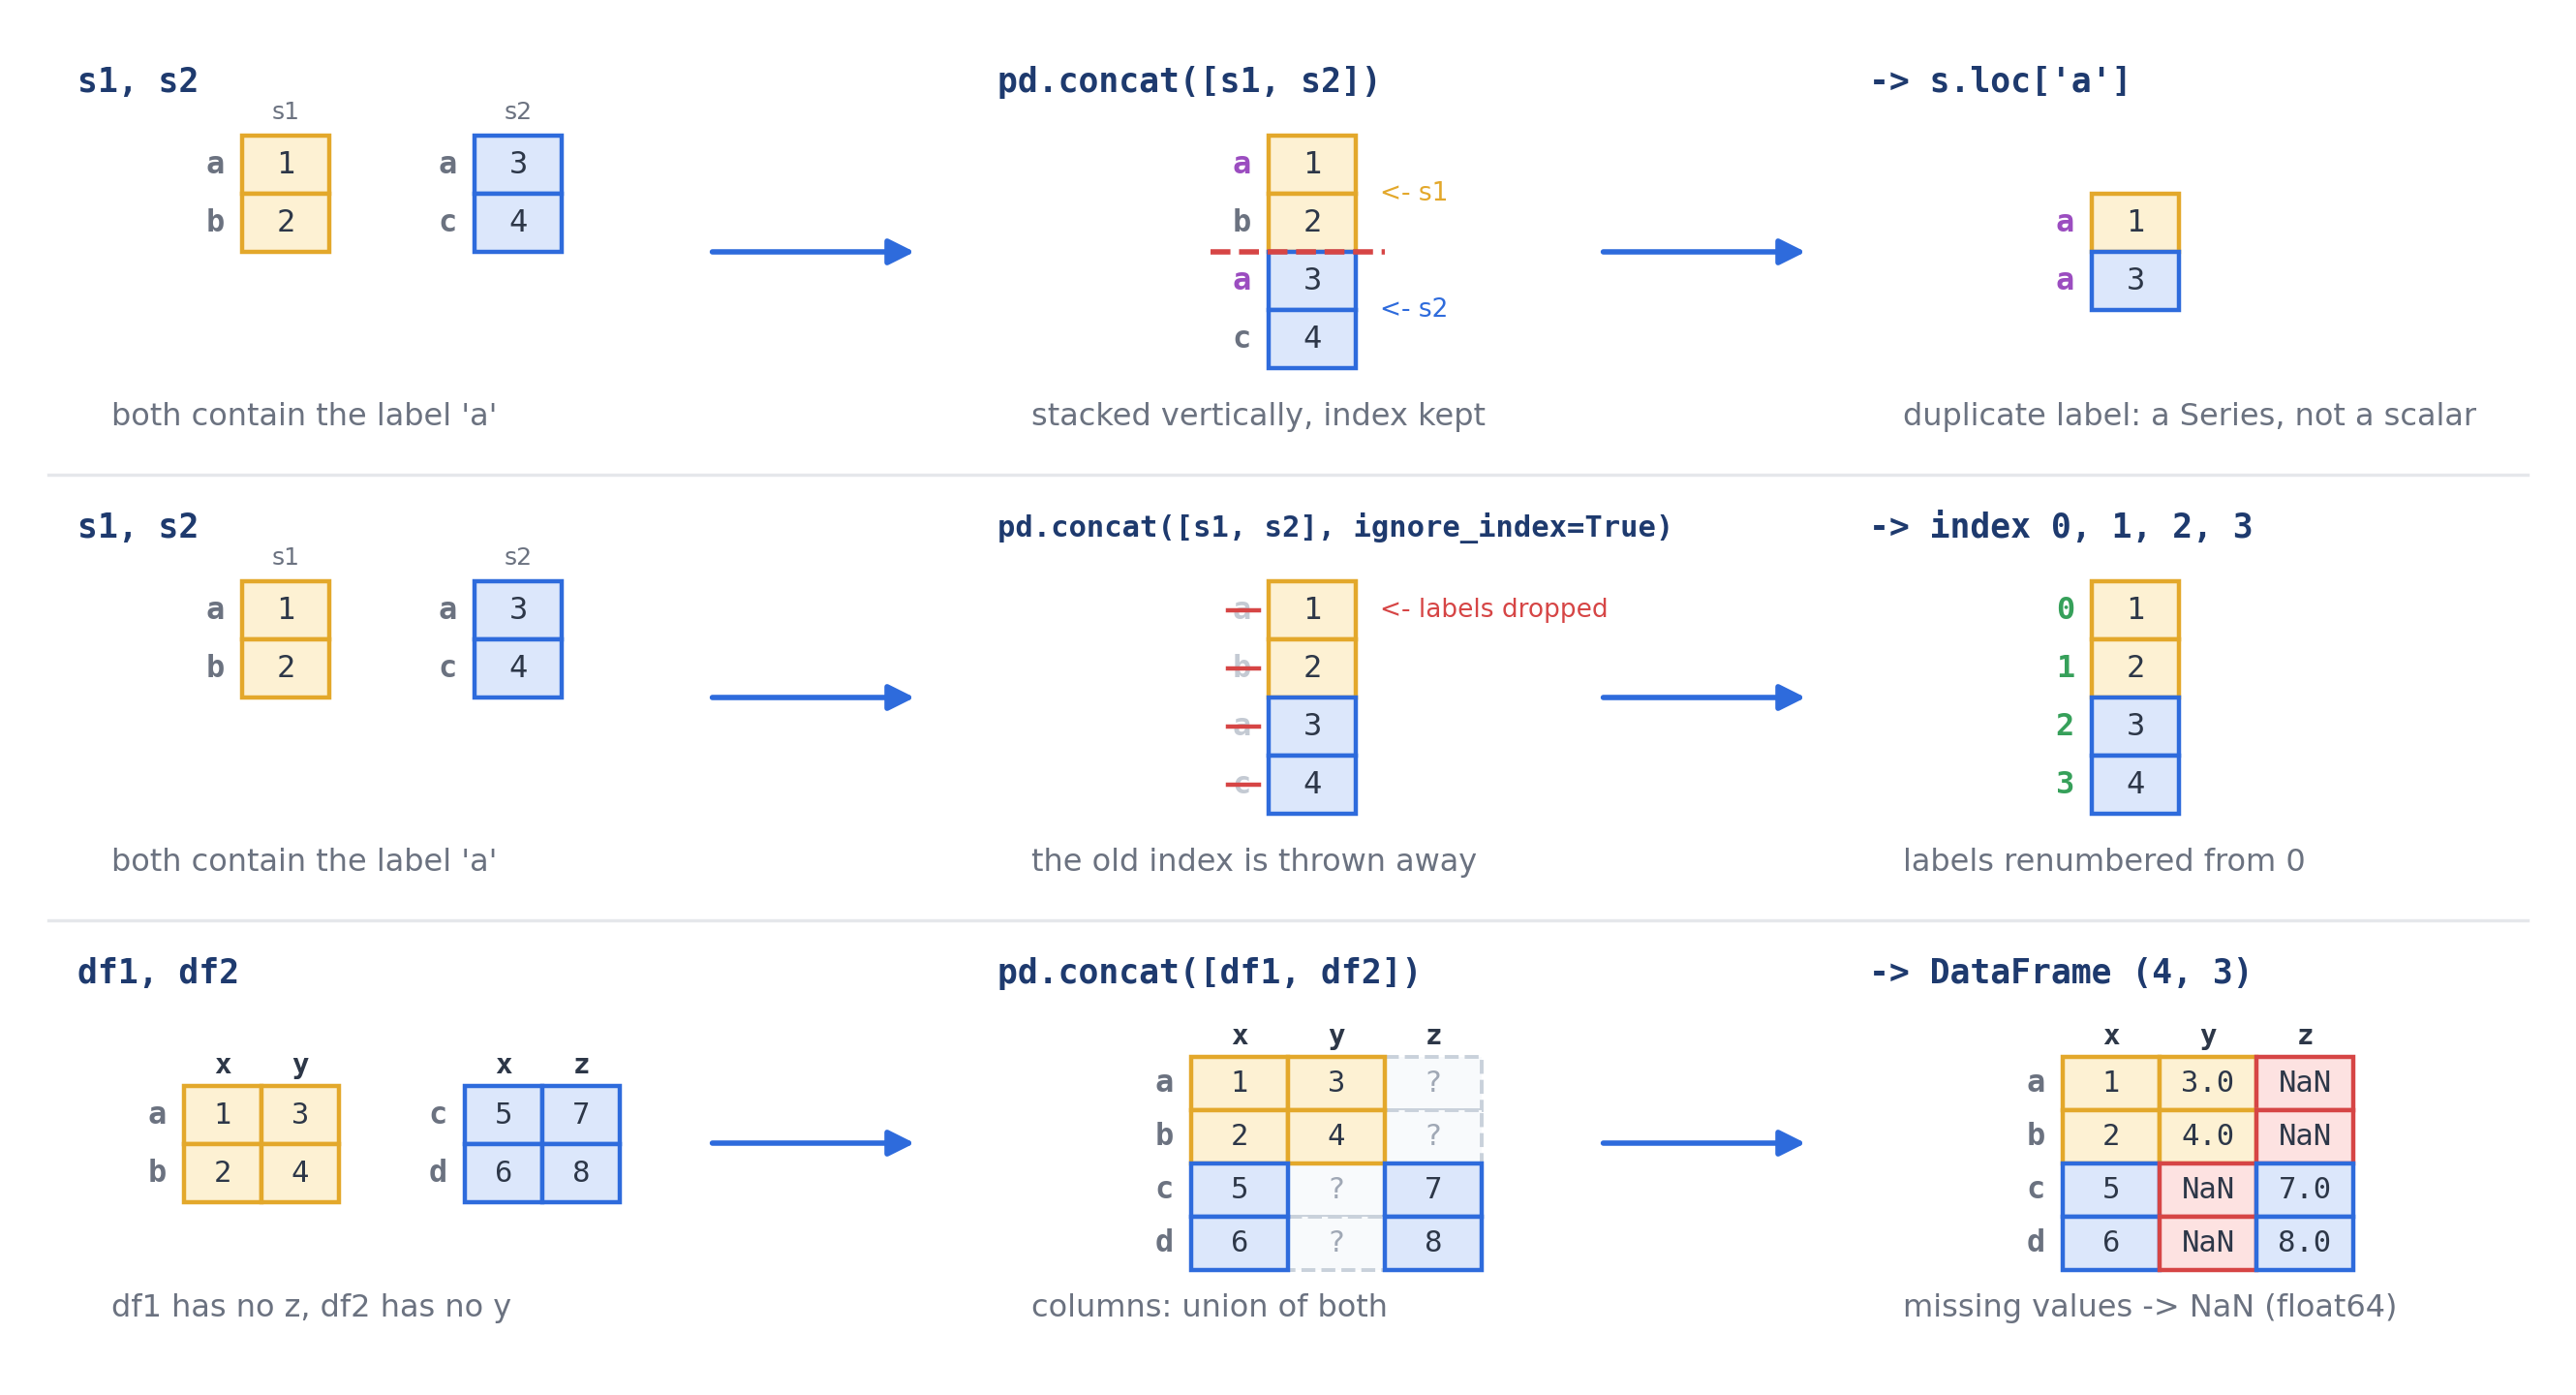
\includegraphics[width=1\textwidth]{contents/images/pandas/sub_concat.png}
    \caption{Concatenation: \texttt{pd.concat} stacks the objects and keeps their labels, so a duplicated label returns several values with \texttt{.loc}. With \texttt{ignore\_index=True} the result is renumbered from 0. Columns missing in one DataFrame are filled with \texttt{NaN}.}
\end{figure}

\begin{itemize}
    \item \textbf{Index preservation:} Concatenation keeps the original index as it is, including duplicate labels. If a label is duplicated, selecting it via \texttt{.loc} will return a Series containing all matches instead of a single scalar.
    \item \textbf{Resetting the index:} Passing \texttt{ignore\_index=True} throws the old index away and renumbers the elements sequentially.
    \item \textbf{Missing columns:} When concatenating DataFrames, if one DataFrame lacks a column present in the other, pandas fills the missing values with \texttt{NaN}.
\end{itemize}

\textit{Note:} The old \texttt{df1.append(df2)} method was removed in pandas 2.0; you should always use \texttt{pd.concat} instead.

\subsection{Merge: Joining on Common Values}
\texttt{pd.merge(df1, df2)} combines two DataFrames similarly to a database SQL join.

\begin{figure}[h]
    \centering
    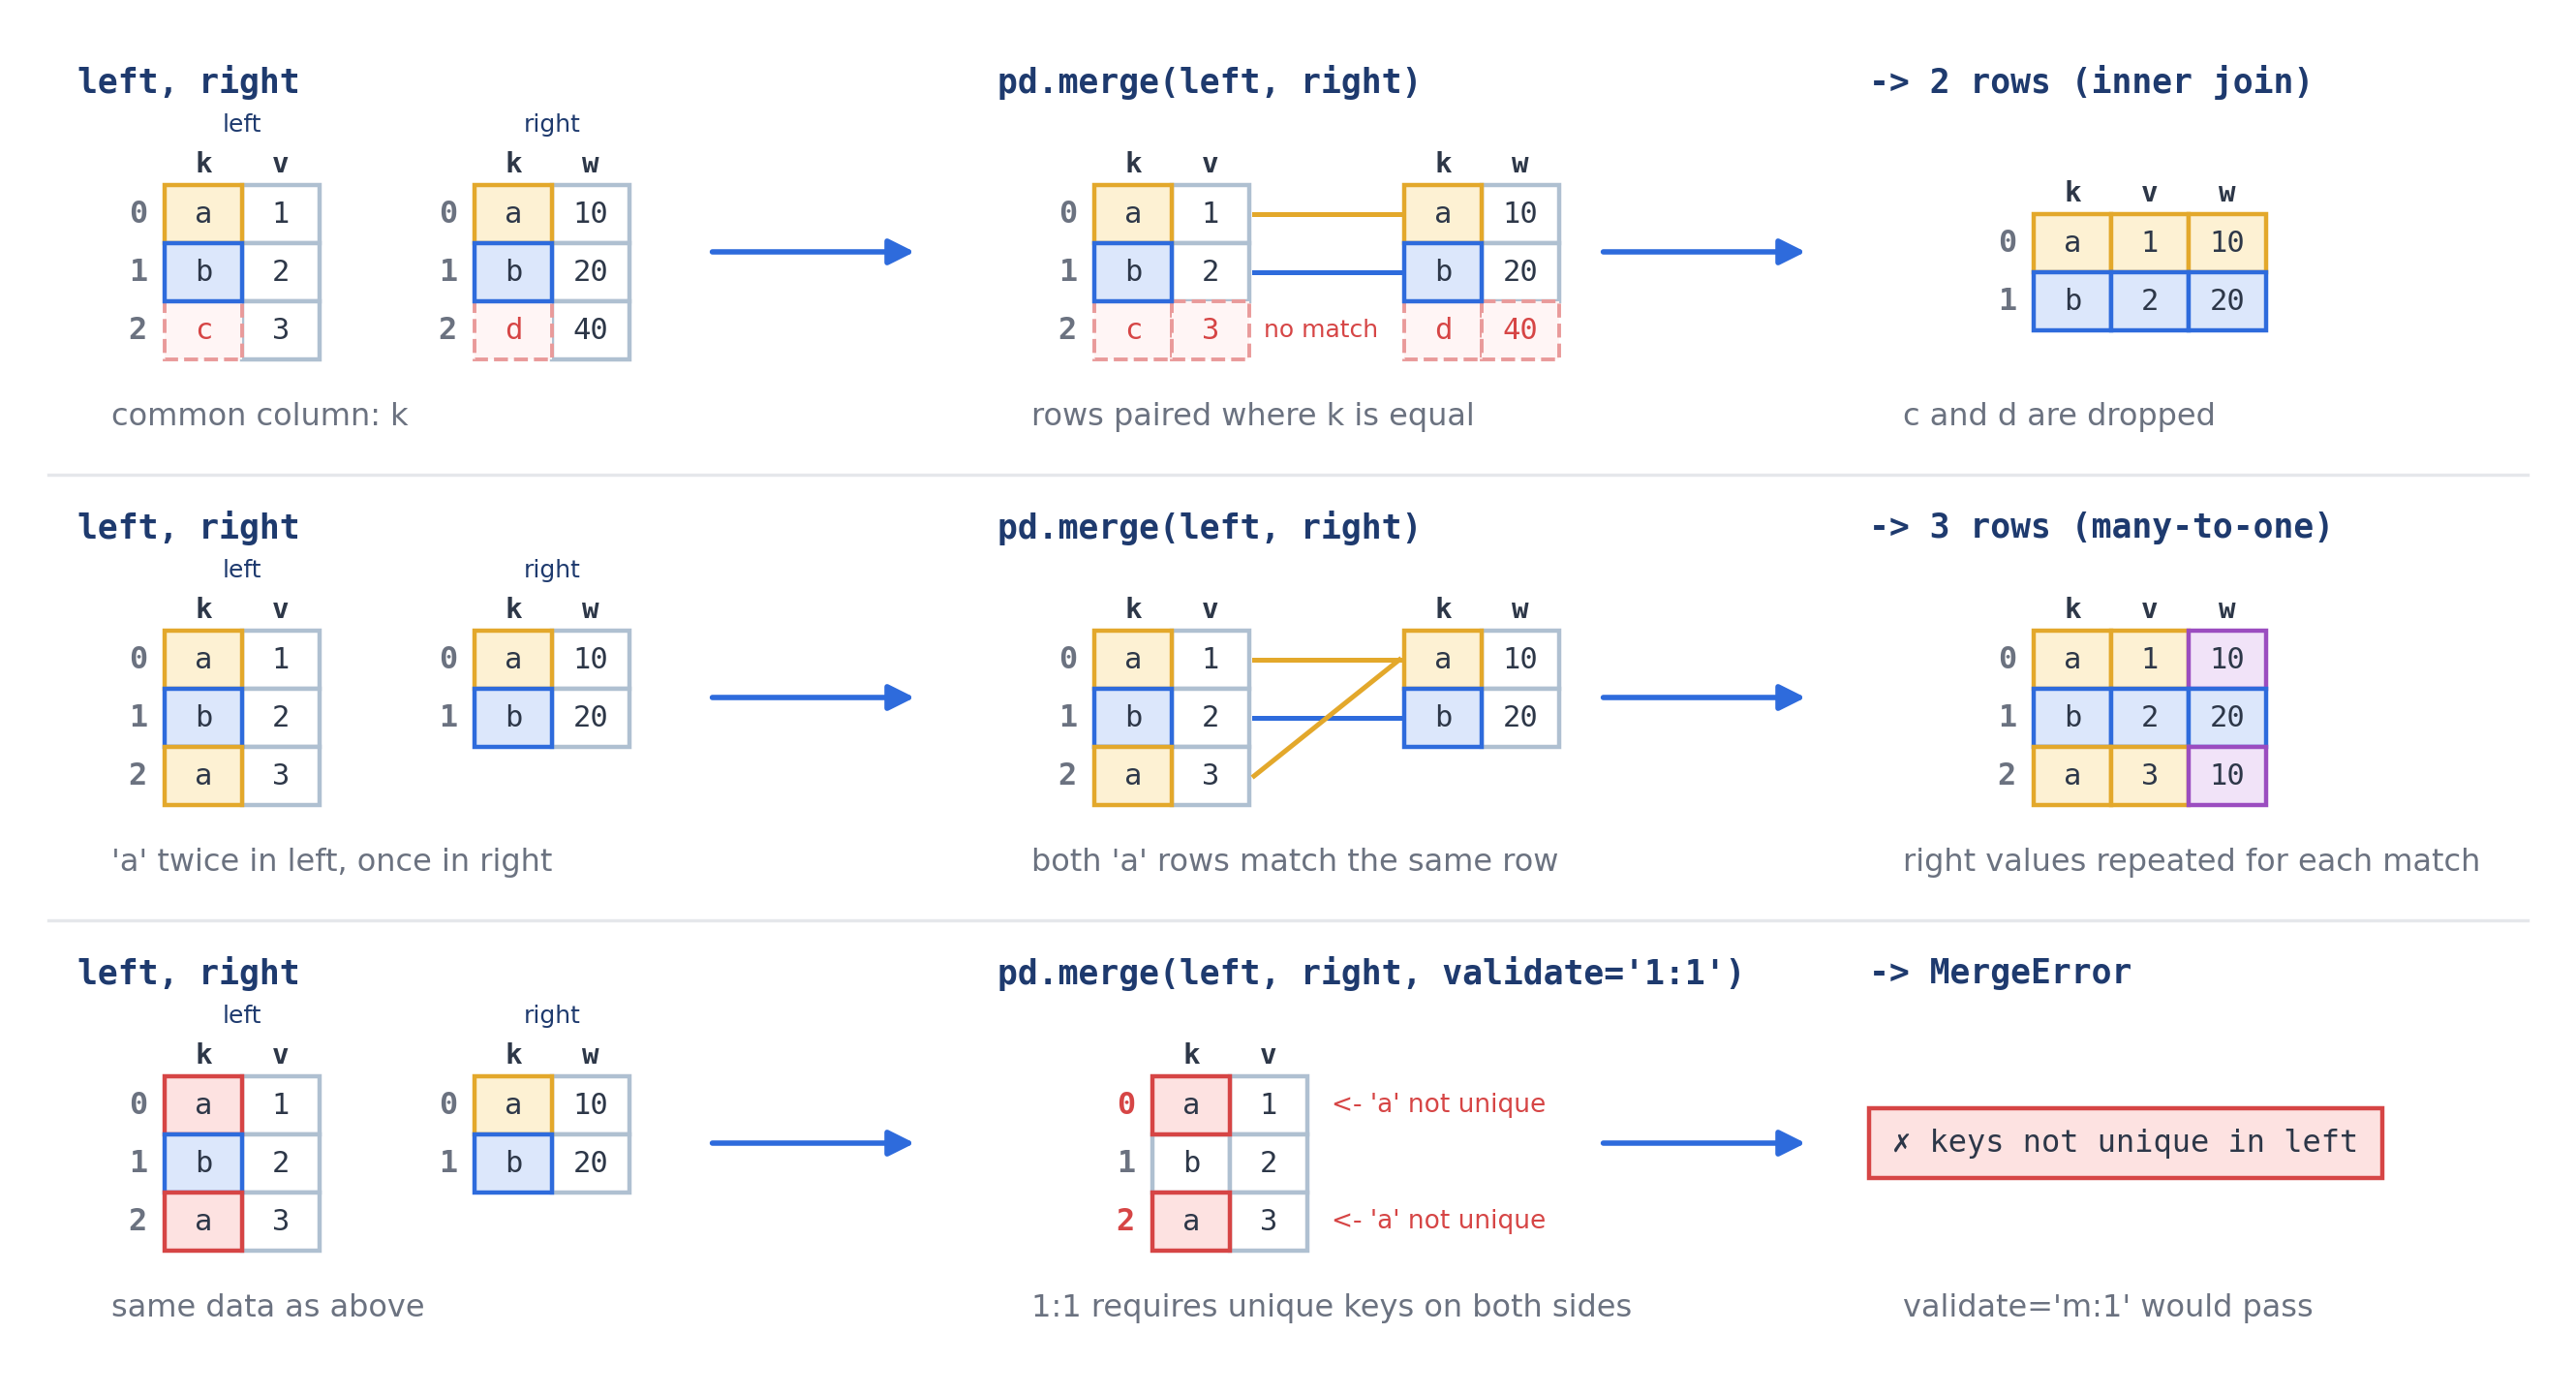
\includegraphics[width=1\textwidth]{contents/images/pandas/sub_merge.png}
    \caption{Merge: rows are paired where the key column \texttt{k} has the same value; by default (inner join) unmatched rows are dropped. In a many-to-one merge the right values are repeated for every matching left row. \texttt{validate='1:1'} raises a \texttt{MergeError} when the keys are not unique.}
\end{figure}

\begin{itemize}
    \item It pairs rows that share equal values in specific columns (by default, columns with the same name, or specified explicitly via \texttt{on=}).
    \item You can also join based on indices using \texttt{left\_index=True, right\_index=True}.
    \item It supports one-to-one, many-to-one, and many-to-many joins. In a many-to-one join, values from the right DataFrame are repeated to match the left.
    \item The \texttt{validate} argument (e.g., \texttt{validate='1:1'}) is used to verify the expected merge type and will raise an error if the data violates this expectation.
\end{itemize}

\lstinputlisting[caption={Concatenating and merging pandas objects.}]{contents/listings/pandas/pandas_combining.py}



\section{Grouping Data}
Pandas provides the equivalent of the SQL \texttt{GROUP BY} statement via \texttt{df.groupby(...)}. This allows you to split the rows into groups by the value of a key column, then iterate, aggregate, or filter the groups.

\subsection{The GroupBy Mechanism}
\begin{figure}[h]
    \centering
    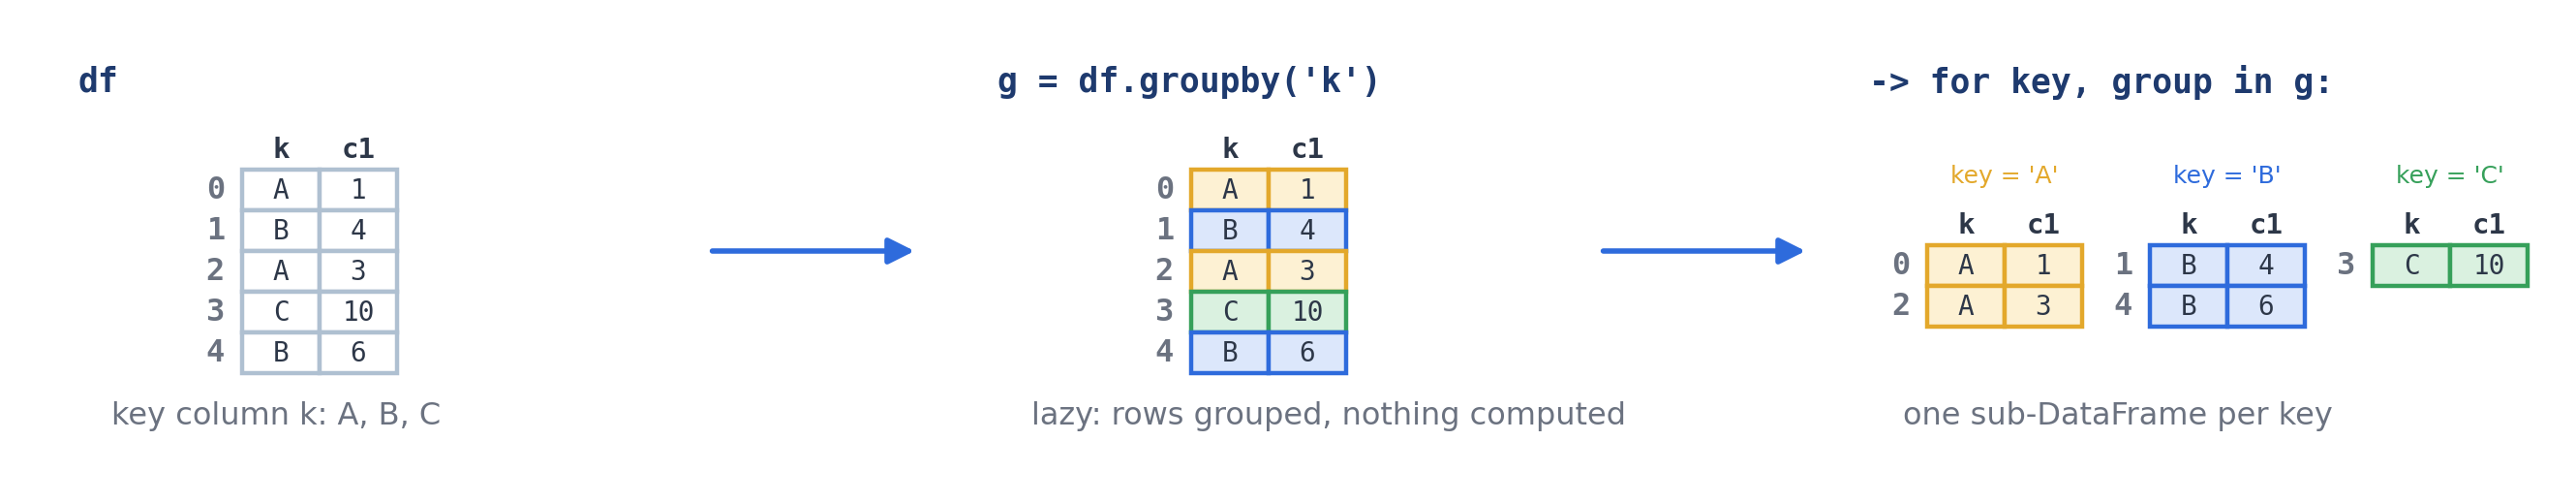
\includegraphics[width=1\textwidth]{contents/images/pandas/sub_groupby_mechanism.png}
    \caption{The GroupBy mechanism: \texttt{df.groupby('k')} only records which rows belong to each key, without computing anything. Iterating over it yields one \texttt{(key, sub-DataFrame)} pair per group, with the original row labels.}
\end{figure}

Calling \texttt{df.groupby("k")} returns a \texttt{DataFrameGroupBy} object, not a computed table; no computation occurs until you explicitly ask for it. You can iterate over this object in a loop, which yields pairs of the group key and a DataFrame subset containing only that group's rows.

\subsection{Aggregating by Group}
When you aggregate a grouped object, the result contains one row per group, and the grouping key becomes the new index.

\begin{figure}[h]
    \centering
    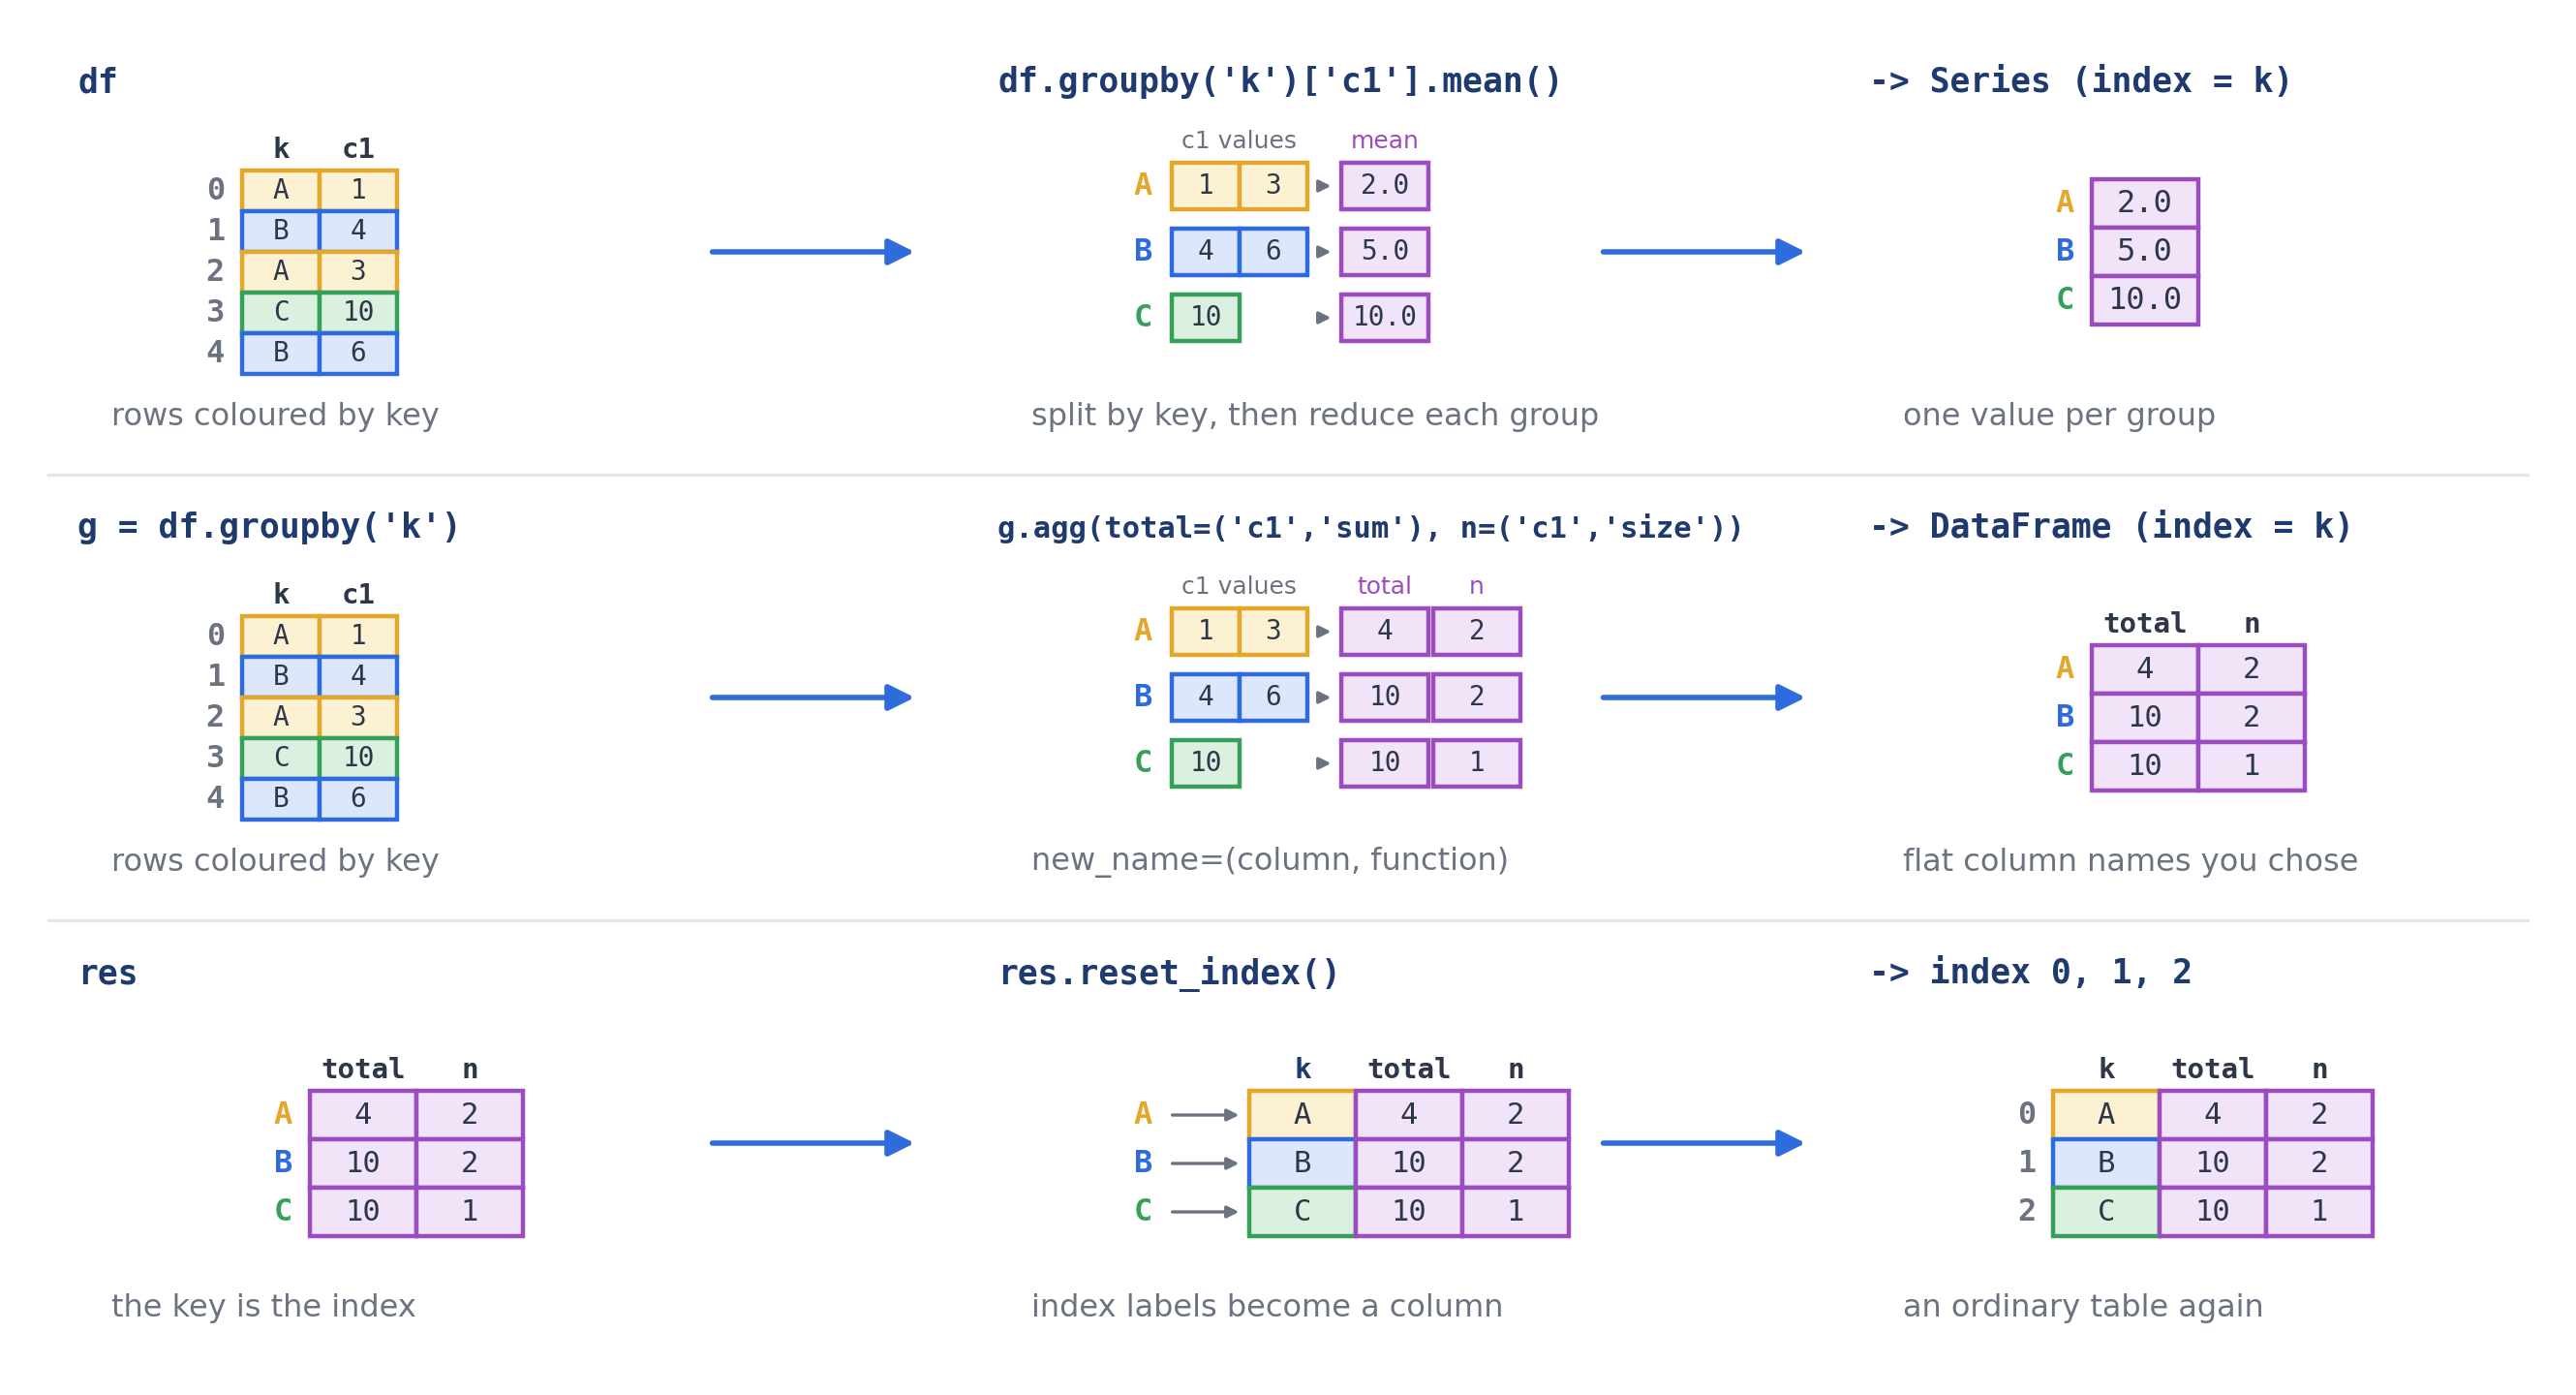
\includegraphics[width=1\textwidth]{contents/images/pandas/sub_groupby_agg.png}
    \caption{Aggregating by group: each group is reduced to one row and the key becomes the index. Named aggregation (\texttt{new\_name=(column, function)}) gives flat column names, and \texttt{reset\_index()} turns the key back into an ordinary column.}
\end{figure}

\begin{itemize}
    \item \textbf{Single column:} \texttt{df.groupby('k')['c1'].mean()} returns a Series.
    \item \textbf{All columns:} \texttt{df.groupby('k').mean()} applies the function to every numeric column and returns a DataFrame.
    \item \textbf{Resetting the index:} Appending \texttt{.reset\_index()} turns the grouping key back into an ordinary column, replacing the index with a standard $0, 1, 2\dots$ sequence.
    \item \textbf{Named Aggregation (Best Practice):} When performing multiple aggregations via \texttt{.agg()}, pandas creates multi-level column names. To avoid this, use named aggregations: \texttt{.agg(new\_name=('column', 'function'))} to keep a flat, readable table.
\end{itemize}

\subsection{Filtering Groups}
The \texttt{.filter()} method applies a boolean function to each group. It evaluates the entire group as a DataFrame and either keeps or drops the \textit{whole} group. The output consists of the original rows that passed the test, without collapsing them into a single row per group.

\begin{figure}[h]
    \centering
    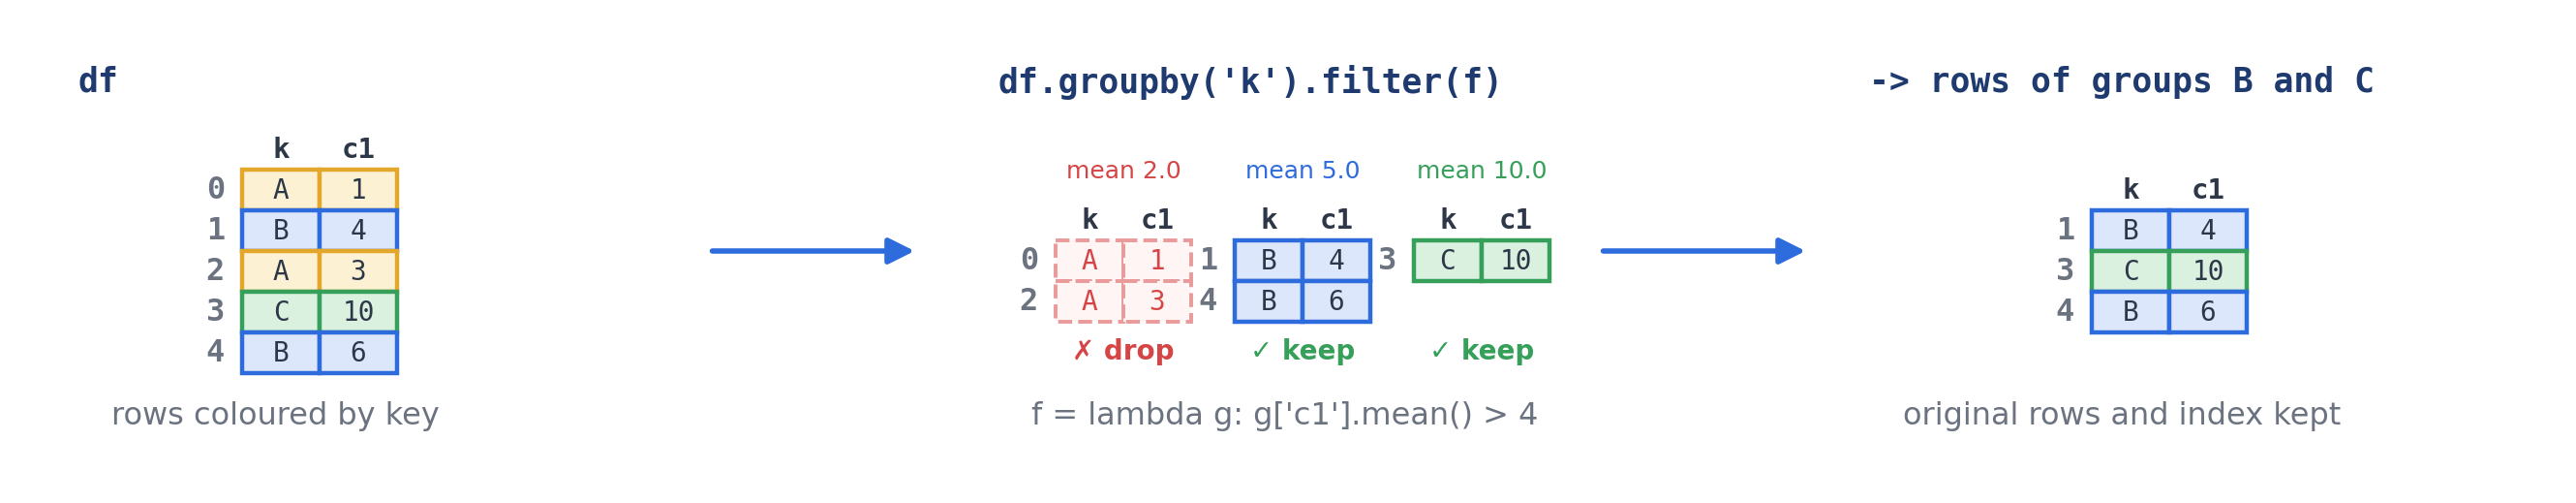
\includegraphics[width=1\textwidth]{contents/images/pandas/sub_groupby_filter.png}
    \caption{Filtering groups: the function receives each group as a DataFrame and returns a single boolean. Whole groups are kept or dropped, and the result contains the original rows with their original index.}
\end{figure}

\lstinputlisting[caption={Grouping, named aggregations, and filtering.}]{contents/listings/pandas/pandas_grouping.py}



\section{DataFrames and I/O}

\subsection{Reading and Writing CSV Files}

\begin{figure}[h]
    \centering
    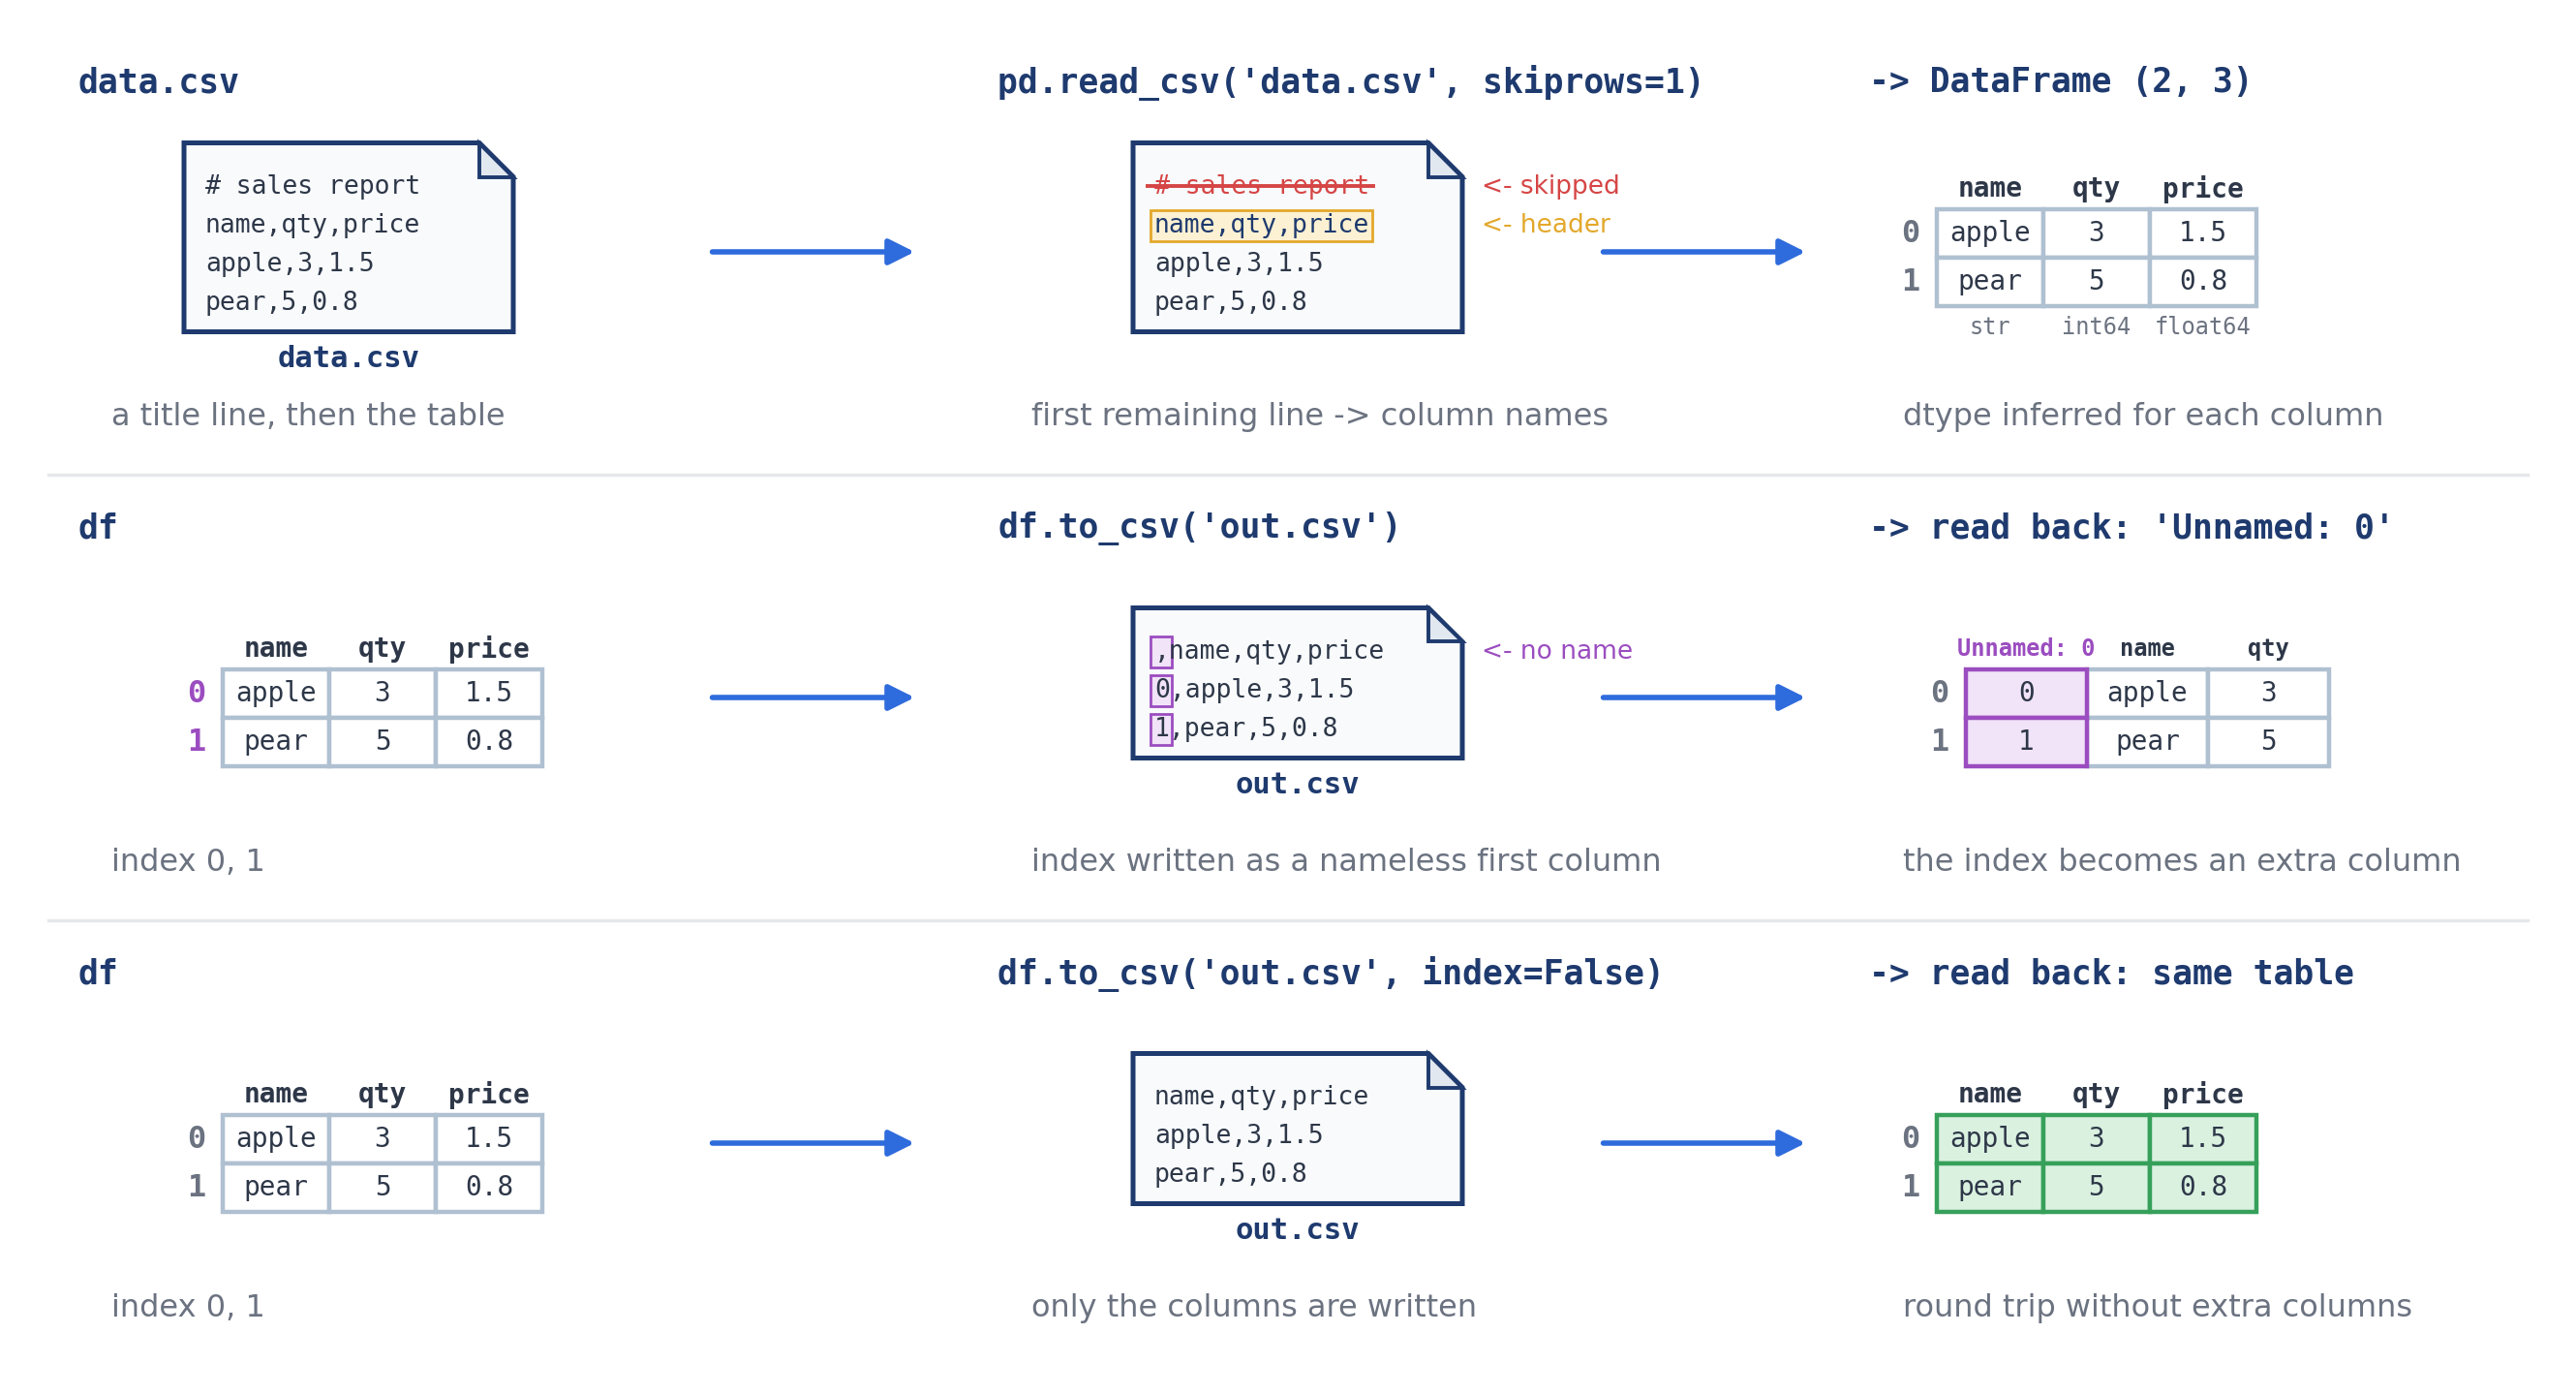
\includegraphics[width=1\textwidth]{contents/images/pandas/sub_csv_io.png}
    \caption{CSV input and output: \texttt{read\_csv} takes the column names from the first line not skipped by \texttt{skiprows} and infers a \texttt{dtype} for each column. By default \texttt{to\_csv} also writes the index as a nameless first column, which comes back as \texttt{Unnamed: 0}; \texttt{index=False} writes only the columns.}
\end{figure}

\begin{itemize}
    \item \textbf{Reading:} \texttt{pd.read\_csv(path, sep=',')} automatically reads column names from the first line and infers the data type of each column. Use \texttt{skiprows=N} to ignore file headers or titles.
    \item \textbf{Writing:} \texttt{df.to\_csv(path)} writes the table to disk. By default, it writes the index as a nameless first column. To omit the index, use \texttt{index=False}.
\end{itemize}

\subsection{Handling Missing Values on Import}
Empty fields and the explicit text "NaN" are automatically converted to \texttt{NaN} upon reading. However, custom missing value markers (e.g., "no info", "x") will cause pandas to read the entire column as text (dtype \texttt{str} or \texttt{object}). To properly parse these and retain numeric types, provide a list of custom markers to the \texttt{na\_values} argument during import.

\begin{figure}[h]
    \centering
    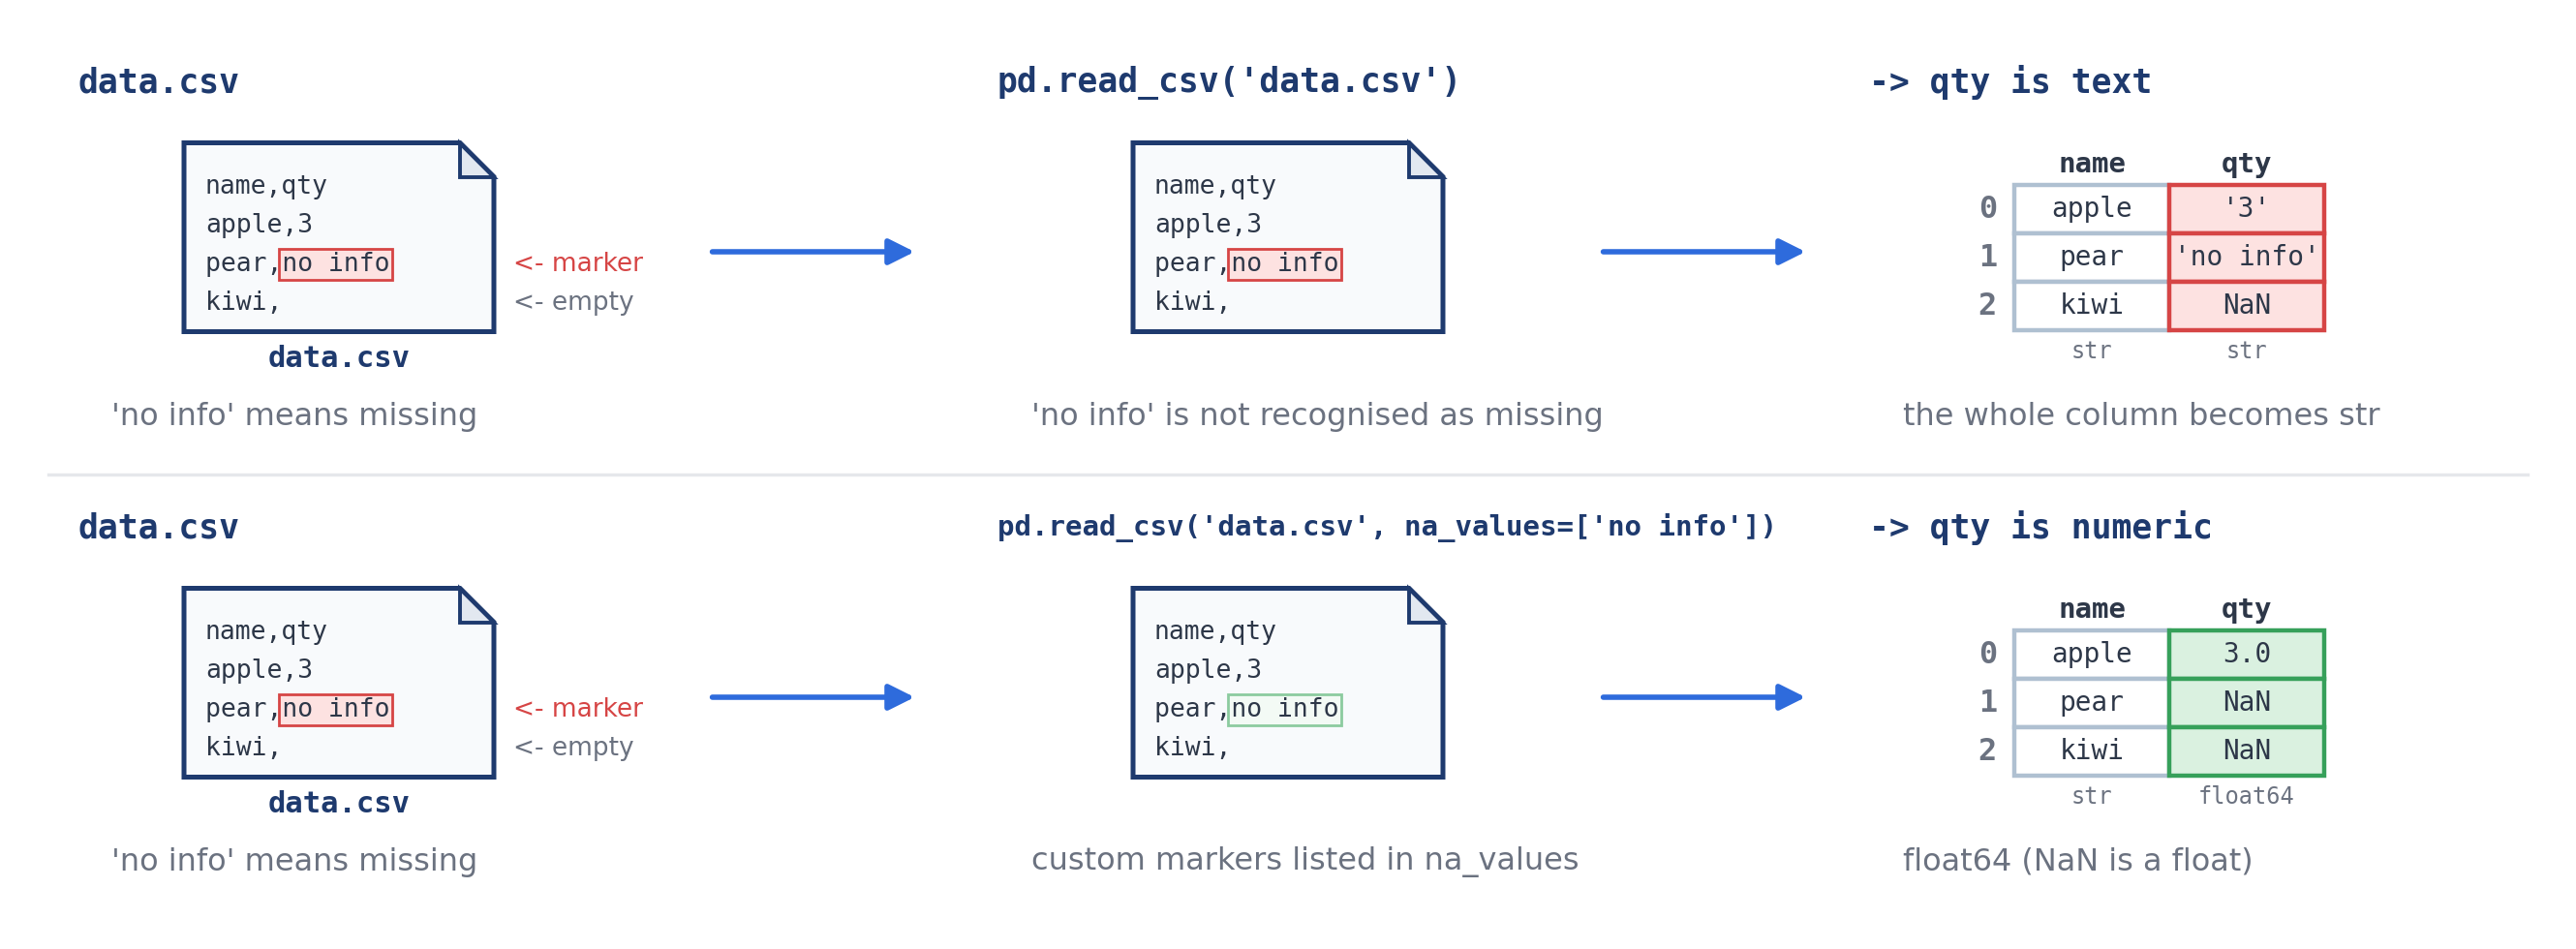
\includegraphics[width=1\textwidth]{contents/images/pandas/sub_missing_values.png}
    \caption{Missing values on import: a custom marker such as \texttt{'no info'} is read as text and turns the whole column into \texttt{str}; listing it in \texttt{na\_values} converts it to \texttt{NaN}, and the column becomes \texttt{float64}.}
\end{figure}

\subsection{Other Supported Formats}
pandas natively supports a wide variety of formats:

\begin{itemize}
    \item \textbf{JSON:} \texttt{pd.read\_json()} and \texttt{df.to\_json}.
    \item \textbf{Excel:} \texttt{pd.read\_excel()} and \texttt{df.to\_excel()}.
    \item \textbf{Parquet:} \texttt{pd.read\_parquet()} and \texttt{df.to\_parquet()} (highly efficient, compressed, and strictly typed, ideal for large datasets).
\end{itemize}

\begin{figure}[h]
    \centering
    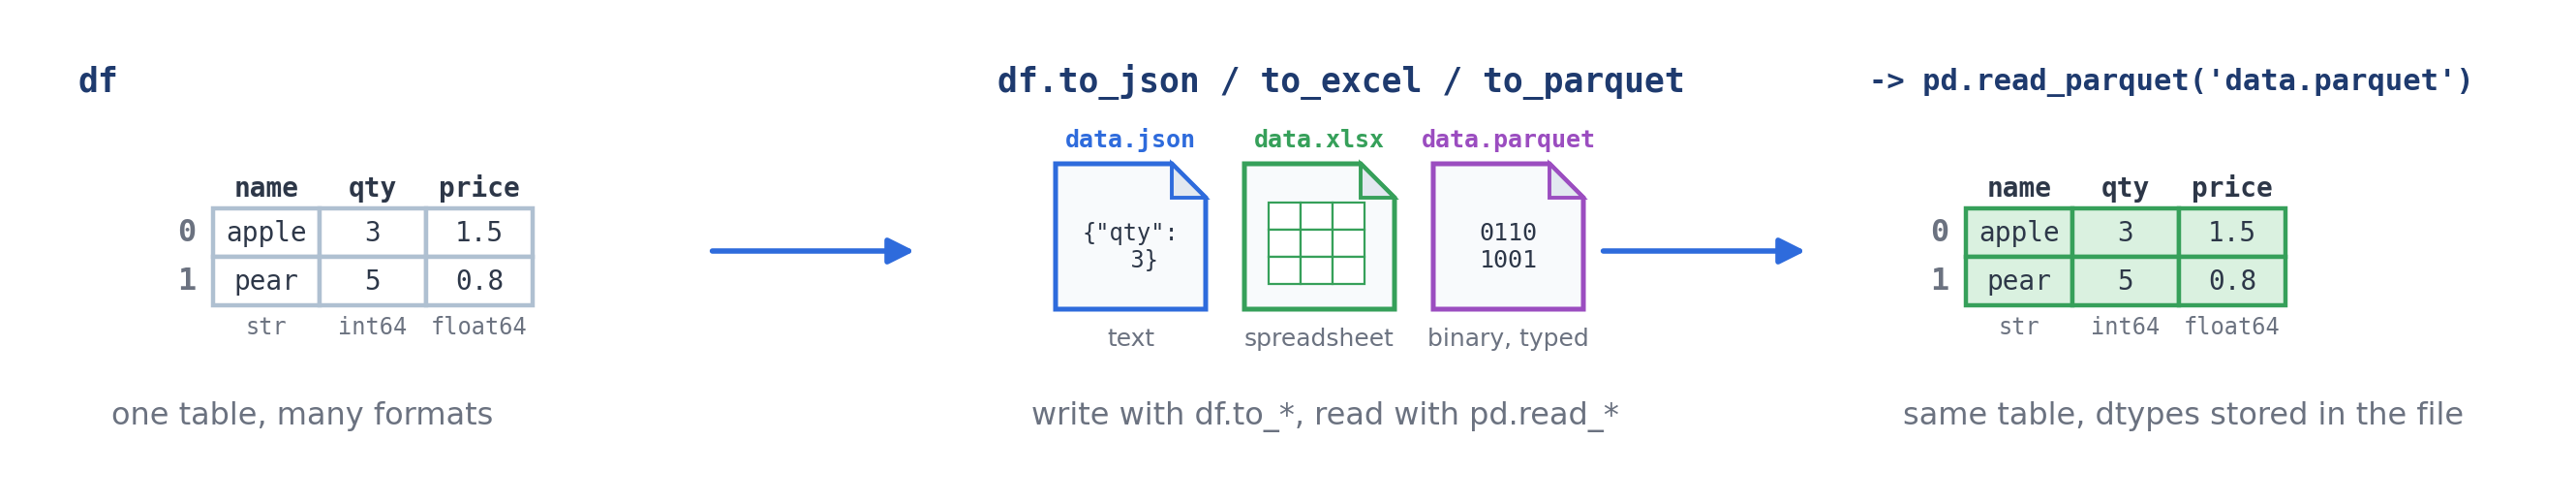
\includegraphics[width=1\textwidth]{contents/images/pandas/sub_formats.png}
    \caption{Other formats: every \texttt{df.to\_*} writer has a matching \texttt{pd.read\_*} reader. JSON is plain text, Excel is a spreadsheet, and Parquet is a compressed binary format that also stores the \texttt{dtype} of each column.}
\end{figure}

\lstinputlisting[caption={Reading and writing CSV files, handling custom missing values.}]{contents/listings/pandas/pandas_io.py}



\section{Missing Values}
Missing data is a common occurrence in real-world datasets (e.g., a sensor failing to answer, an empty field in a file, or a merge with no match). pandas marks these missing values with \texttt{NaN} (Not a Number), and it also accepts standard Python \texttt{None} values, automatically converting them to \texttt{NaN}. 
Because \texttt{NaN} is technically a floating-point value, introducing it into a column of integers will upcast the entire column to \texttt{float64}, allowing the numbers to remain in a highly optimized NumPy array.

\subsection{Detecting, Dropping, and Filling}
pandas provides several methods to handle missing data. It is important to note that \textbf{none of these methods modify the original object}; each returns a new Series or DataFrame.

\begin{figure}[h]
    \centering
    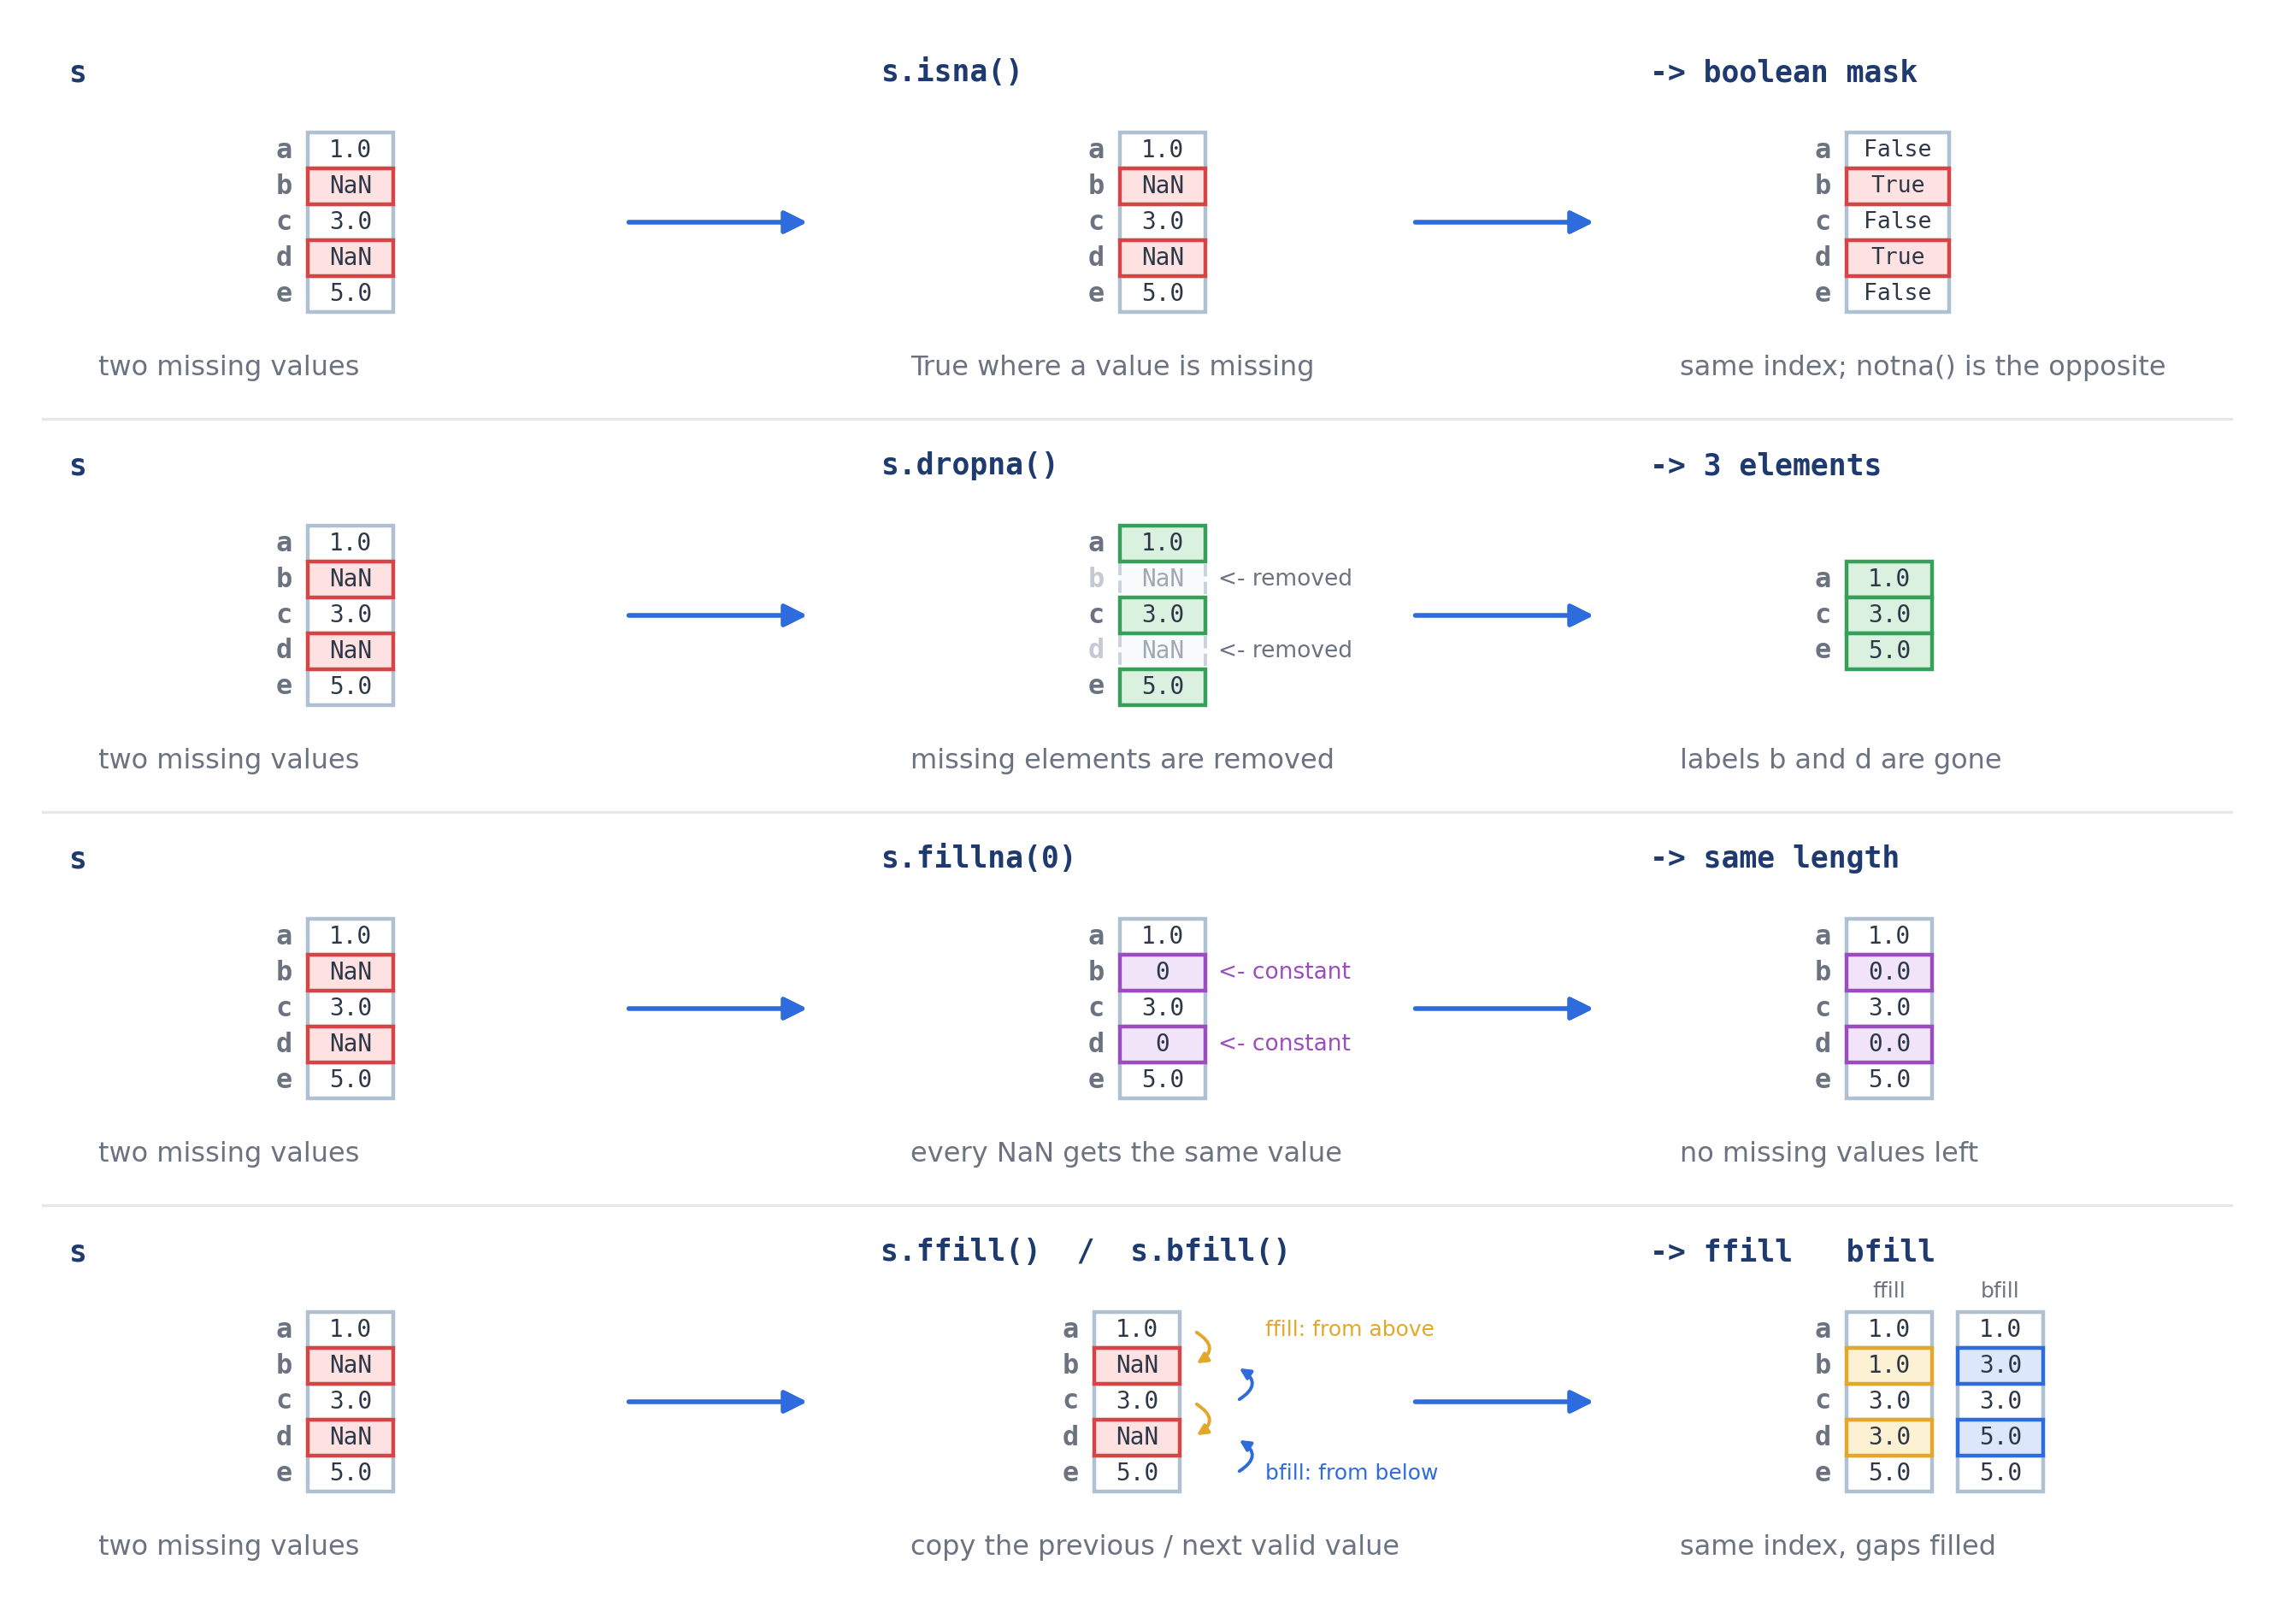
\includegraphics[width=1\textwidth]{contents/images/pandas/sub_missing_series.png}
    \caption{Missing values in a Series: \texttt{isna()} marks them with \texttt{True}, \texttt{dropna()} removes them together with their labels, \texttt{fillna(0)} replaces them with a constant, and \texttt{ffill()}/\texttt{bfill()} copy the previous or next valid value. Each method returns a new object.}
\end{figure}

\begin{itemize}
    \item \textbf{Detecting:} \texttt{isna()} (and its opposite, \texttt{notna()}) returns a boolean mask of the exact same shape, containing \texttt{True} wherever a value is missing.
    \item \textbf{Dropping:} \texttt{dropna()} completely removes the missing elements.
    \item \textbf{Filling with a constant:} \texttt{fillna(value)} replaces every missing value with the specified \texttt{value} (e.g., \texttt{0}).
    \item \textbf{Forward/Backward filling:} \texttt{ffill()} replaces every missing value with the previous valid one, while \texttt{bfill()} uses the next valid one.
\end{itemize}

\subsection{Missing Values in a DataFrame}
When dealing with a 2-dimensional DataFrame, \texttt{dropna()} drops entire rows that contain at least one missing value. 

\begin{figure}[h]
    \centering
    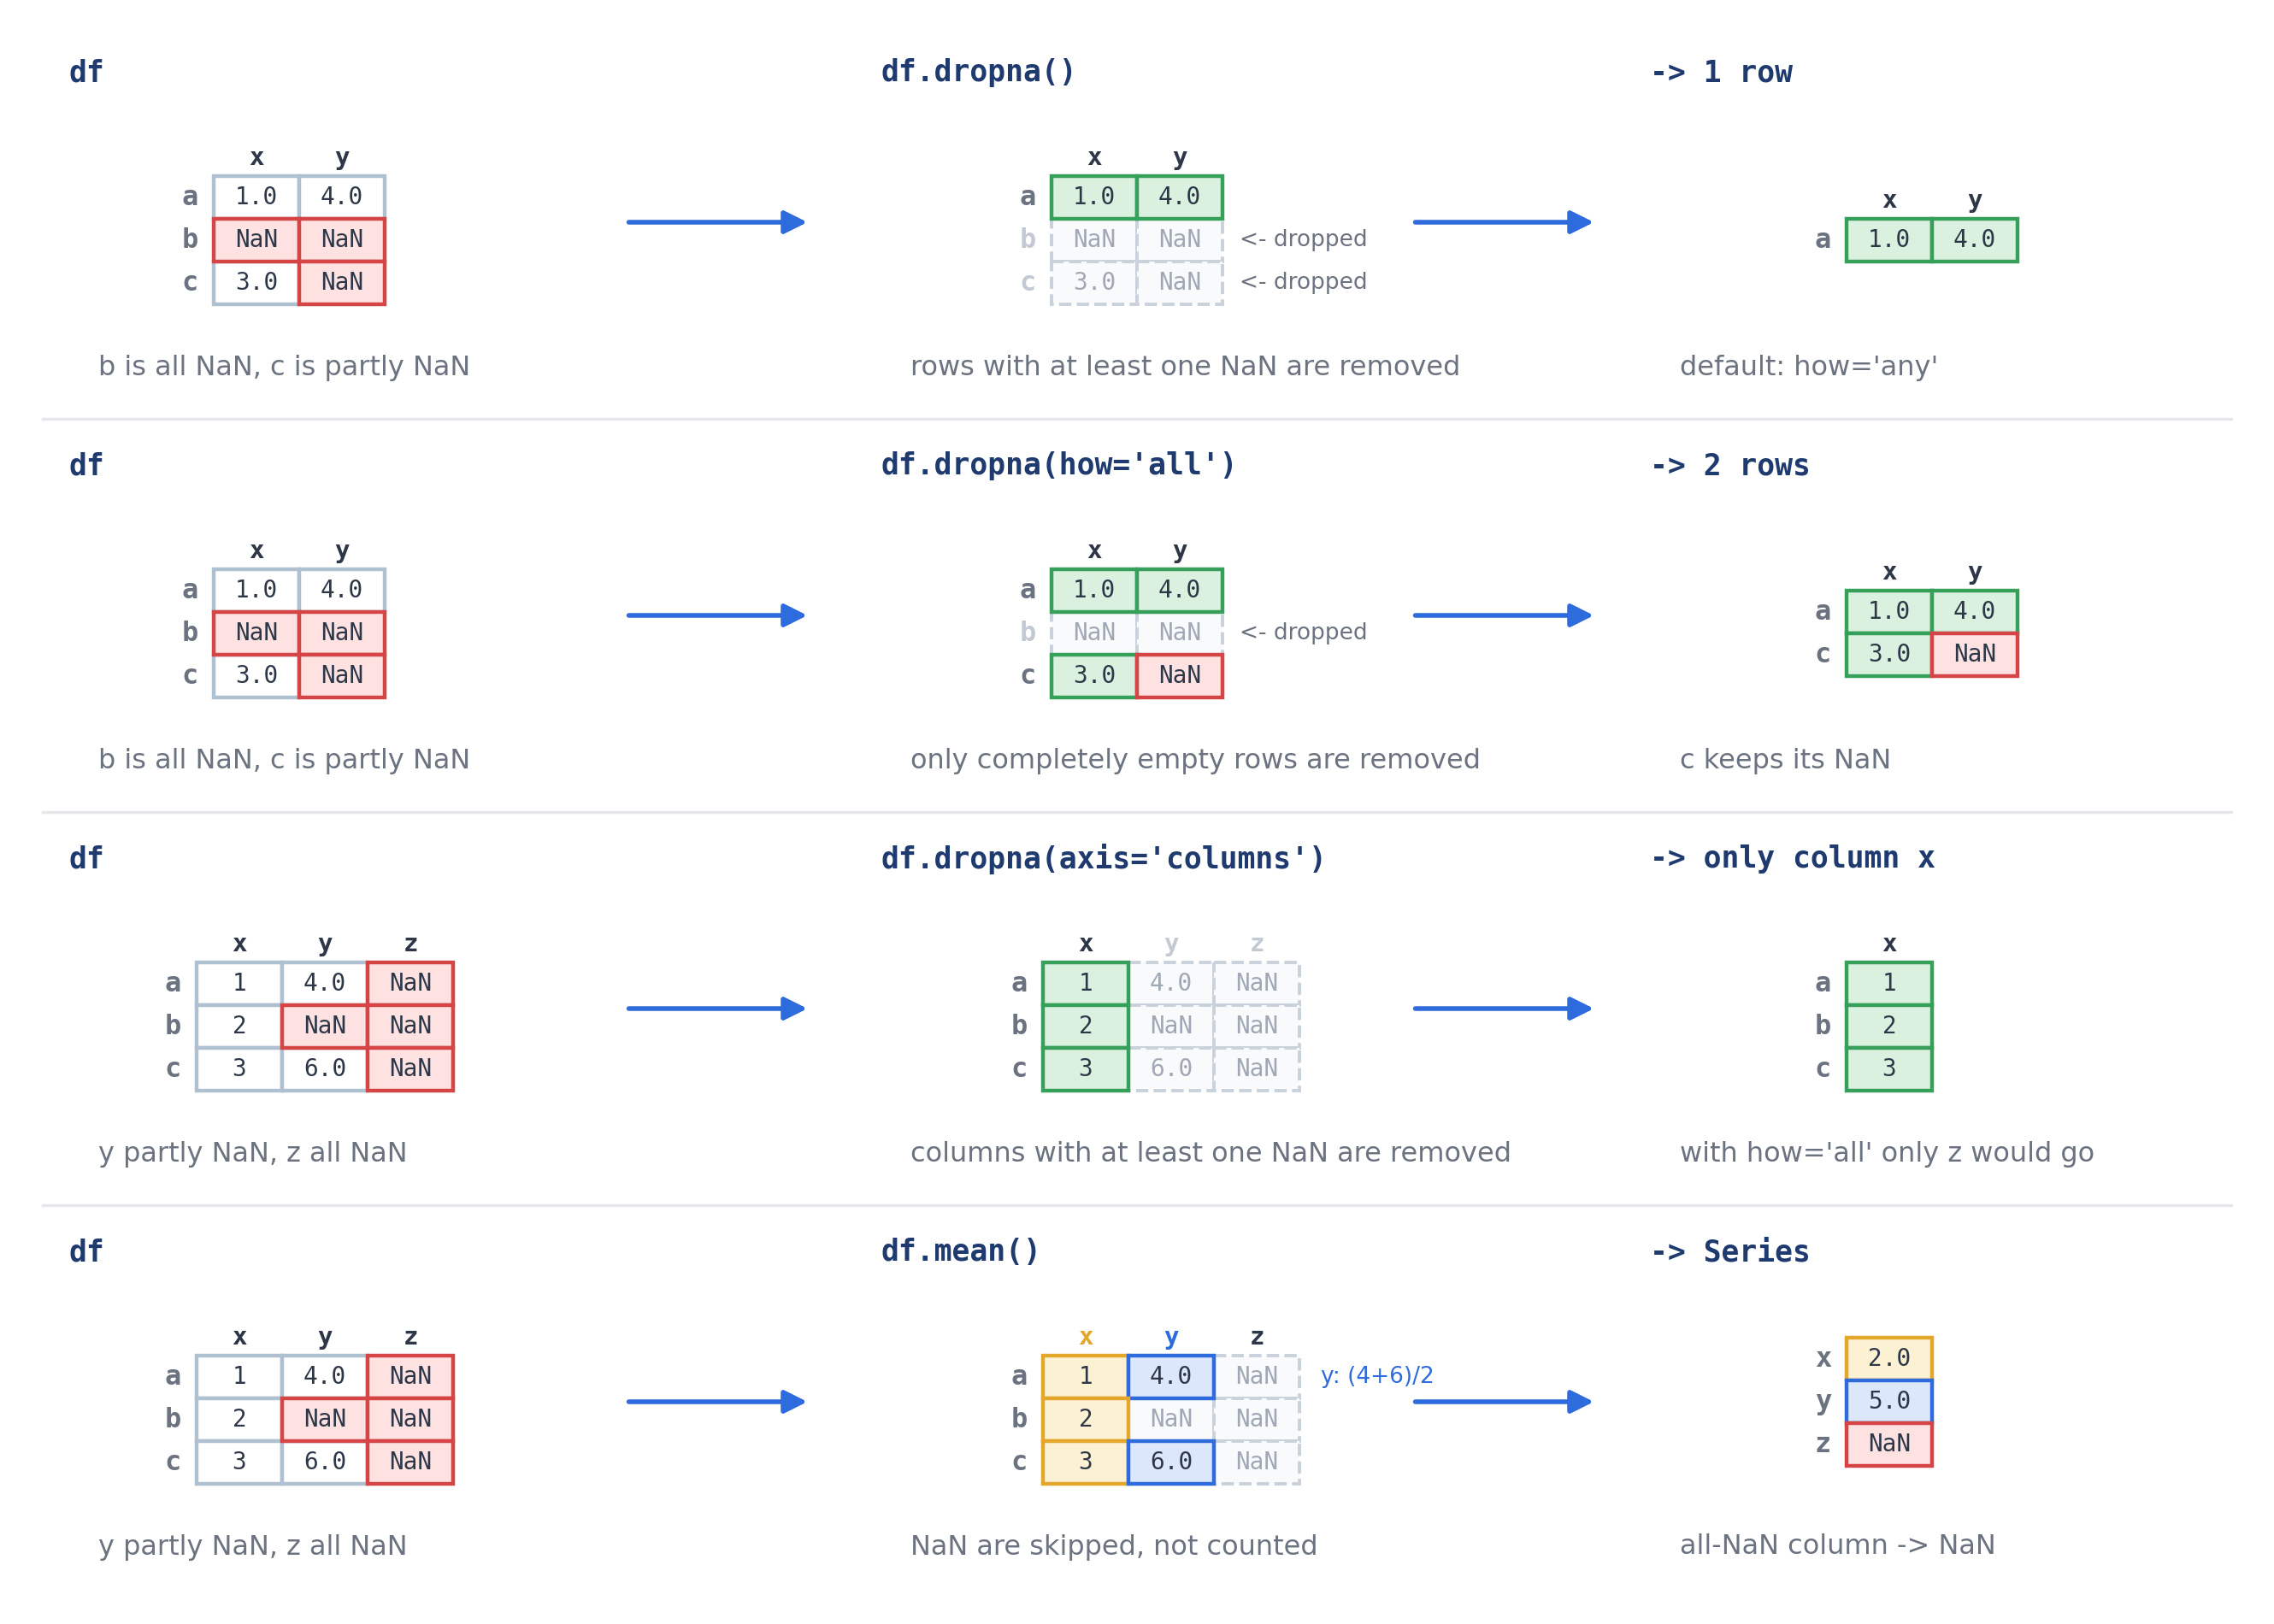
\includegraphics[width=1\textwidth]{contents/images/pandas/sub_missing_dataframe.png}
    \caption{Missing values in a DataFrame: \texttt{dropna()} removes every row with at least one \texttt{NaN}, \texttt{how='all'} only the completely empty ones, and \texttt{axis='columns'} works on columns instead. Aggregations such as \texttt{mean()} skip \texttt{NaN}; a column with no valid values gives \texttt{NaN}.}
\end{figure}

\begin{itemize}
    \item You can change this behavior to drop columns instead by using \texttt{axis='columns'}. 
    \item If you only want to drop rows/columns that are entirely empty, use the \texttt{how='all'} argument.
\end{itemize}
Finally, when performing aggregations (like \texttt{.mean()} or \texttt{.sum()}), pandas automatically skips \texttt{NaN} values by default, computing the result using only the existing data points.

\lstinputlisting[caption={Handling missing values in Series and DataFrames.}]{contents/listings/pandas/pandas_missing_values.py}
